\documentclass{article}
\usepackage{graphicx,color}
\usepackage{parskip}
\usepackage{placeins}
\usepackage[font={small,it}]{caption}
\begin{document}

Jan, Joachim has run a bunch of simulations and we have looked through them in order to find a reasonable story. 
Joachim, I already lost the sketch due to moving between offices etc. In planned to write this in google
docs, but was not able to upload the pdfs as images.  

Anyway, here goes the story. 


\begin{figure}
\begin{center}
\includegraphics[page=24,width=\linewidth]{../../doc/presentation.pdf}
\caption{2D spinal cord problem. The parameters are as shown in the figure, except that $b=0$ everywhere (giving $\tau\rightarrow\infty$), and $\Delta t=10^{-3}$.}
\end{center}
\end{figure}

\begin{figure}
\begin{center}
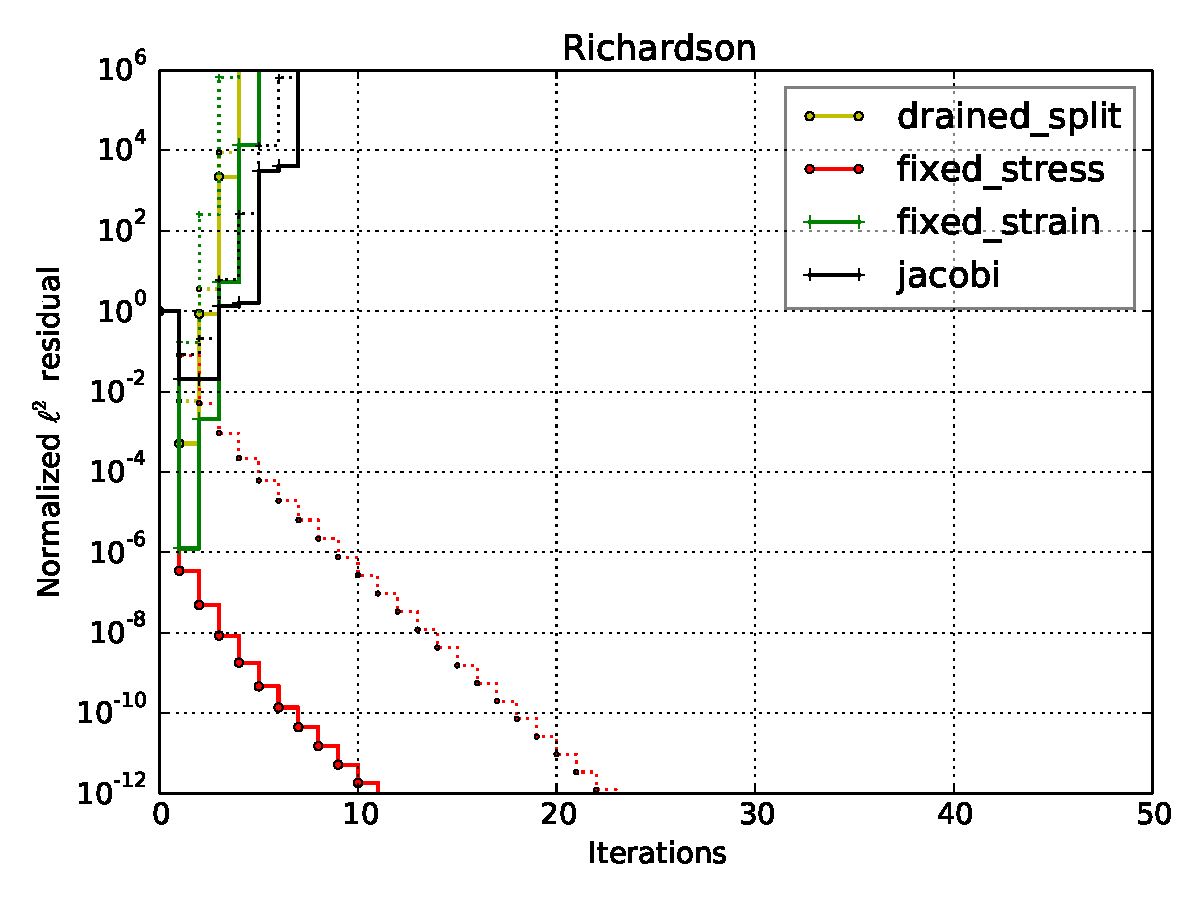
\includegraphics[width=0.49\linewidth]{../Richardson,problem=2,exact=1,N=64.pdf}
\caption{Richardson iterations (exact subsolves) is equivalent to the traditional splitting schemes. The residual is shown as solid lines; energy-norm error as dotted lines. Coupling strength $\tau\rightarrow\infty$ when $b\rightarrow 0$, so the unstable splittings diverge quickly. (Undrained split is not included in the comparison, because it is undefined for $b=0$.)} 
\label{2dsc-richardson-exact}
\end{center}
\end{figure}

\begin{figure}
\begin{center}
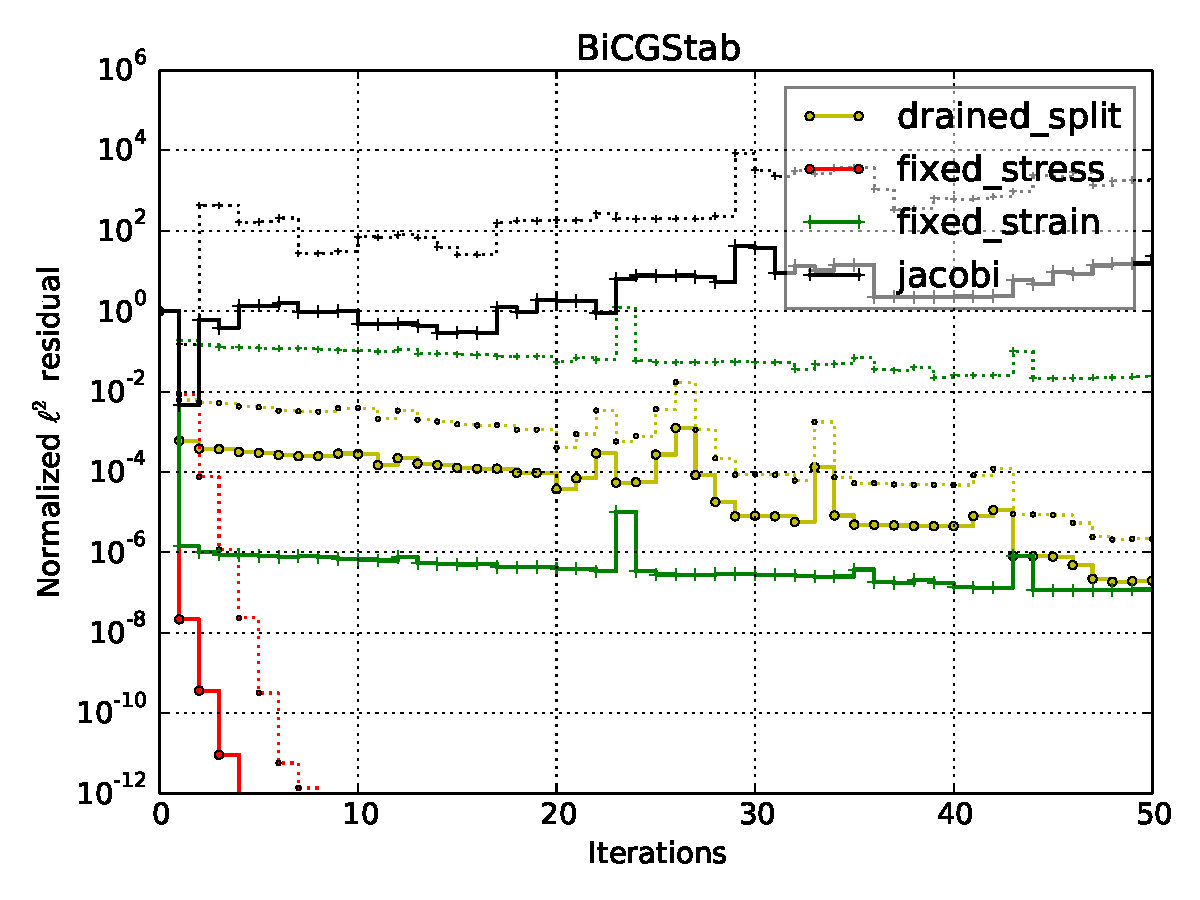
\includegraphics[width=0.49\linewidth]{../BiCGStab,problem=2,exact=1,N=64.pdf}
\includegraphics[width=0.49\linewidth]{../LGMRES,problem=2,exact=1,N=64,cycles=1.pdf}
\caption{BiCGStab and LGMRES (exact subsolves). The residuals is shown as solid lines; energy-norm error as dotted lines. For LGMRES, the energy-norm error is (nearly?) invisible because it overlaps with the residual lines. }
\label{2dsc-bicgstab-lgmres-exact}
\end{center}
\end{figure}

Pictures \ref{2dsc-richardson-exact}--\ref{2dsc-bicgstab-lgmres-exact} shows that Krylov methods are superior to Richardson. This is not a big surprise, but provides
a clear link to the splitting schemes.

\begin{figure}
\begin{center}
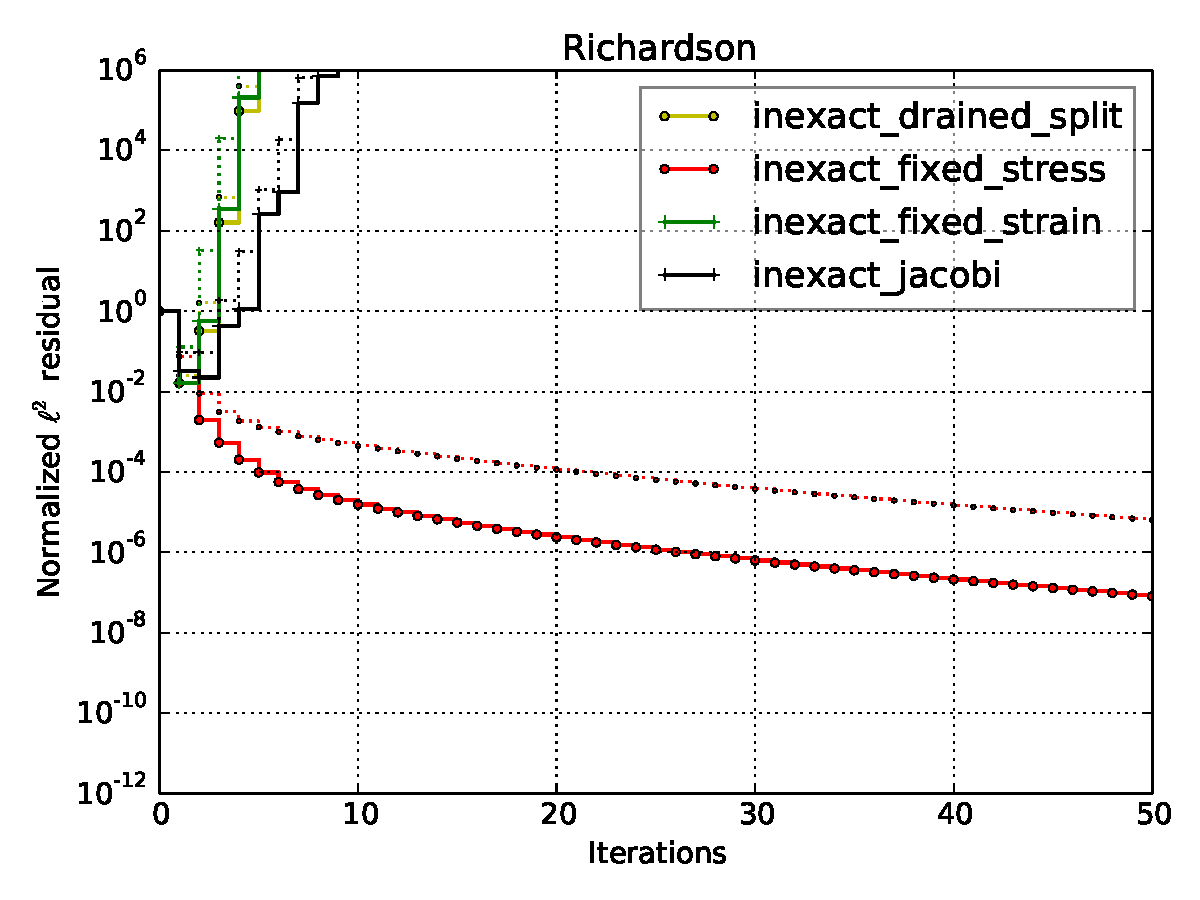
\includegraphics[width=0.32\linewidth]{../Richardson,problem=2,exact=0,N=64.pdf}
\includegraphics[width=0.32\linewidth]{../BiCGStab,problem=2,exact=0,N=64.pdf}
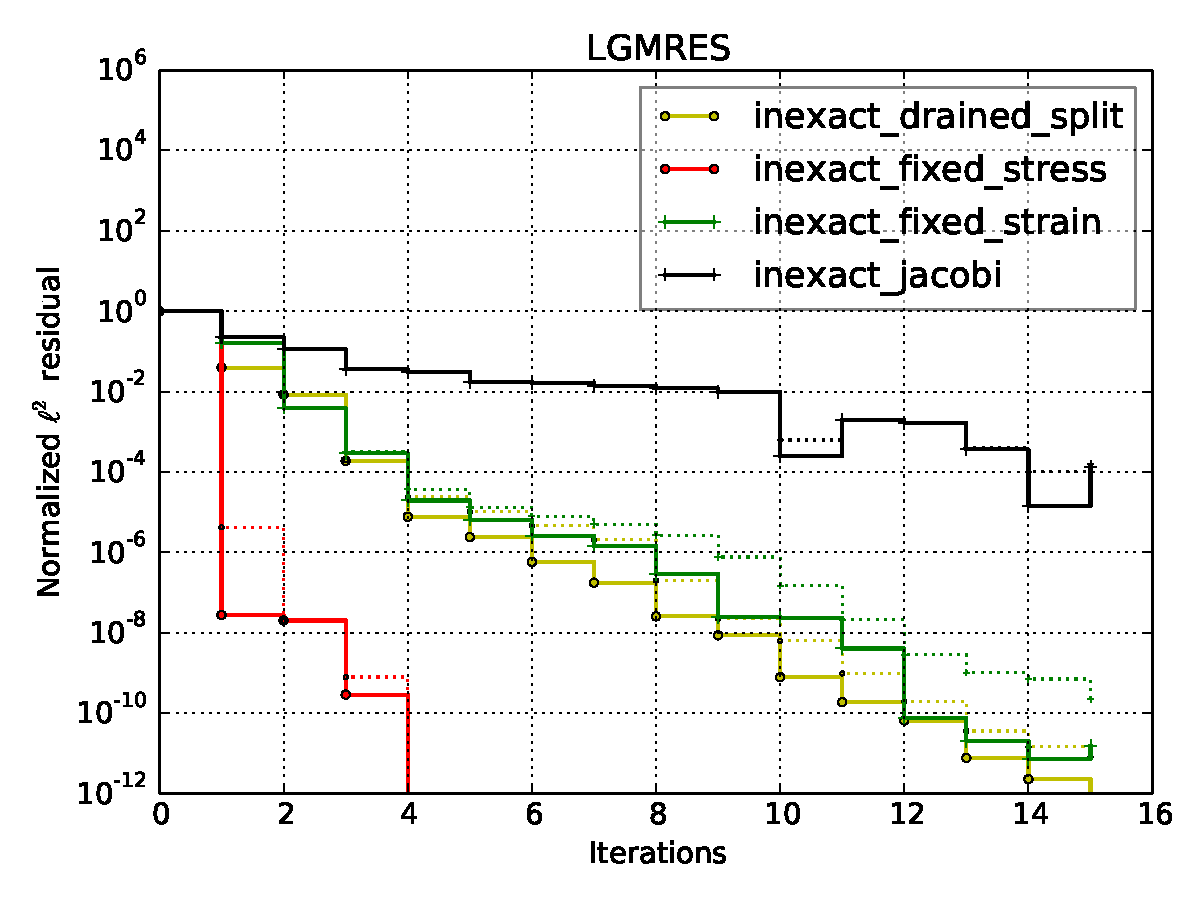
\includegraphics[width=0.32\linewidth]{../LGMRES,problem=2,exact=0,N=64,cycles=1.pdf}
\caption{Richardson and LGMRES with inexact subsolves (1 cycle of ML).} 
\label{2dsc-richardson-lgmres-inexact}
\end{center}
\end{figure}

%\begin{figure}
%\begin{center}
%\includegraphics[width=0.32\linewidth]{../Richardson,problem=2,exact=0,N=64,cycles=2.pdf}
%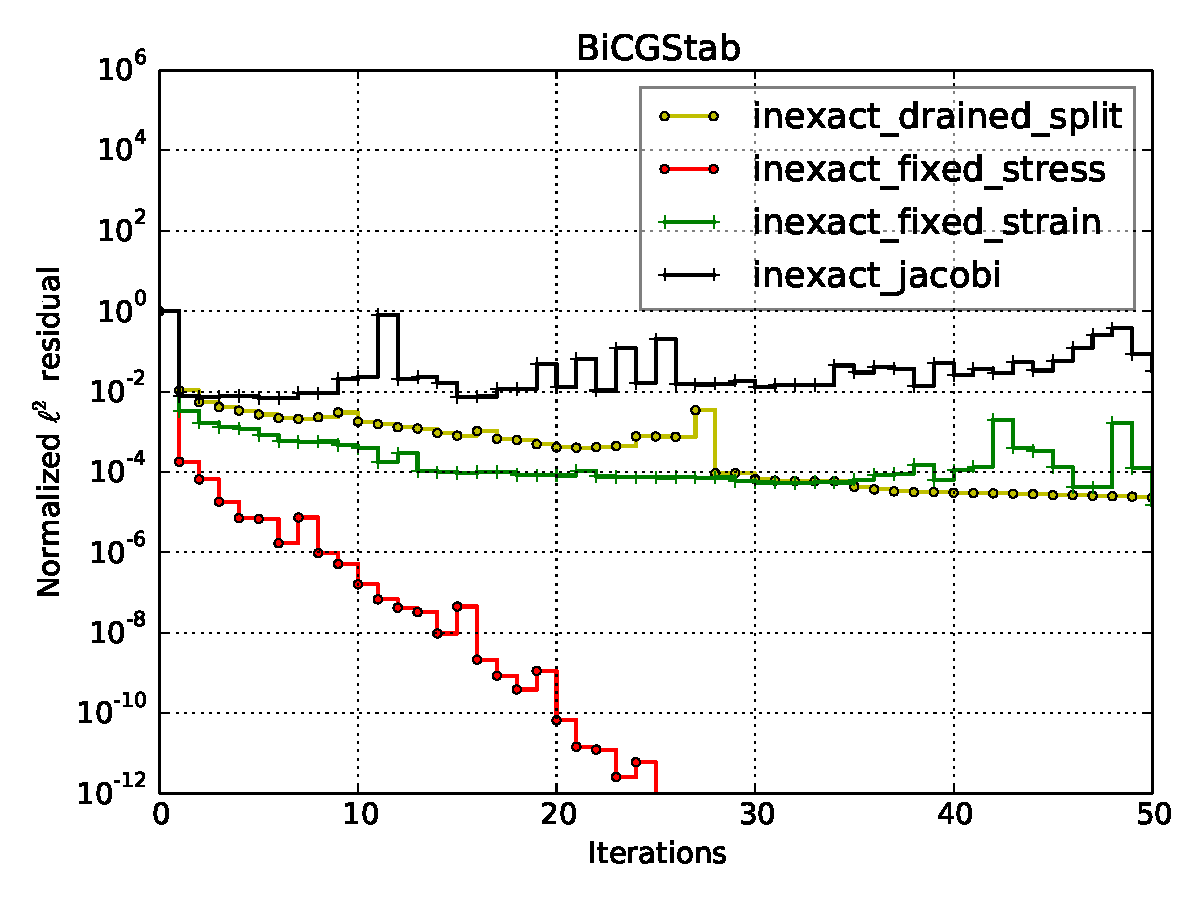
\includegraphics[width=0.32\linewidth]{../BiCGStab,problem=2,exact=0,N=64,cycles=2.pdf}
%\includegraphics[width=0.32\linewidth]{../LGMRES,problem=2,exact=0,N=64,cycles=2.pdf}
%\caption{Richardson and LGMRES with inexact subsolves (2 cycles of ML).} 
%\label{2dsc-richardson-lgmres-inexact-2cycle}
%\end{center}
%\end{figure}

The figures also show both the error (in energy norm) and the residual for BiCGStab and LGMRES. 
Here dotted lines are residual and the solid line is energy. Here, it is clear that it is a
close correspondance between error and residual for LGMRES and less clear for BiCGStab. We therefore
continue the discussion with only LGMRES and error. 

Note to be included in the discussion: 
It is not immediately obvious that the Krylov methods are very
superior. Given that BiCGStab is about twice as expensive per iteration, and
LGMRES is 30+ times as expensive per iteration, they may something like 30\%
faster. What is clear is: (a) They are reasonable preconditioners, compared
to the bog-standard Block Jacobi method; (b) Even the unstable splittings
converge, at least in LGMRES; and (c) Error is much better controlled in
LGMRES than in either Richardson or BiCGStab. In the contrast example
we would expect larger differences between Richardson and Krylov since Krylov
methods may pich up outliers (and there are few in the contrast example). 
At least CG and MinRes has this property. LGMRES and BiCGStab might not. 

Figure \ref{2dsc-richardson-lgmres-inexact} shows that the same pattern holds
when the splitting is performed using inexact single-block solvers.

\emph{Further note (JBH): I have made a new plot that is perhaps more persuasive, shown in figure~\ref{new-2dsc-inexact}. Here, the number of iterations for each method is tuned so that the full number of iterations take about the same for all methods.}

Next, lets consider the eigenvalues of the individual components. 
\begin{figure}
\begin{center}
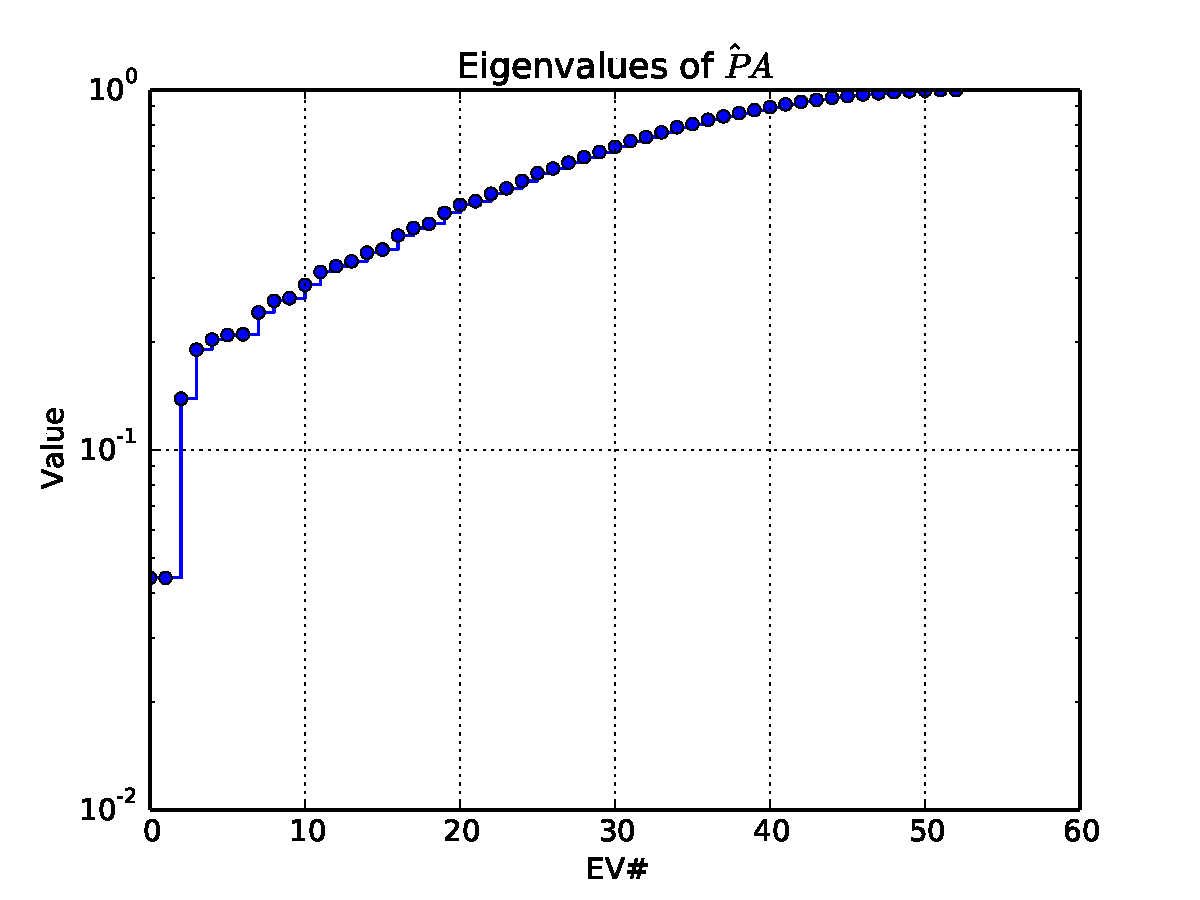
\includegraphics[width=.49\linewidth]{../EV[A],problem=2,exact=0,N=32.pdf}
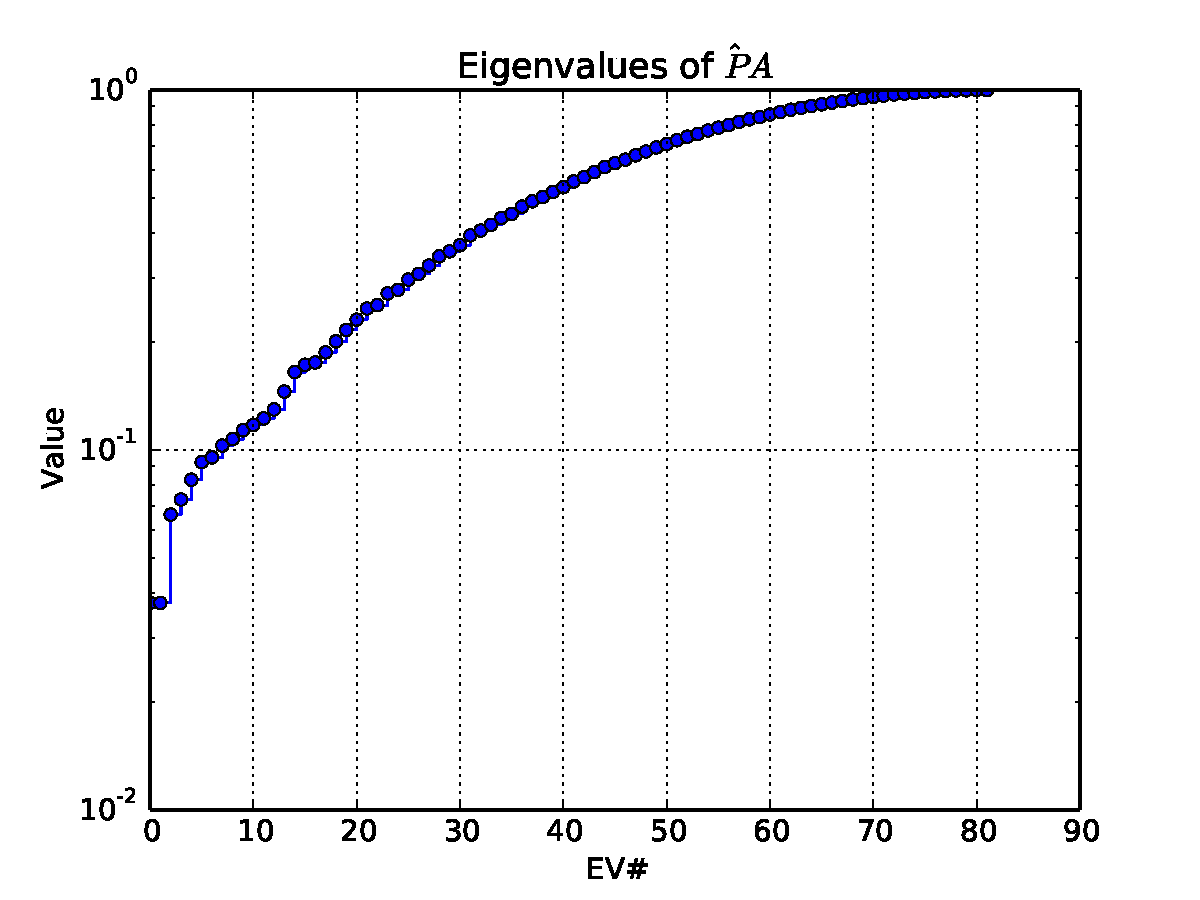
\includegraphics[width=.49\linewidth]{../EV[A],problem=2,exact=0,N=64.pdf}
\caption{Eigenvalues of the preconditioned $A$ block at $N=32$ (left) and $N=64$ (right).}
\label{evA}
\end{center}
\end{figure}

\begin{figure}
\begin{center}
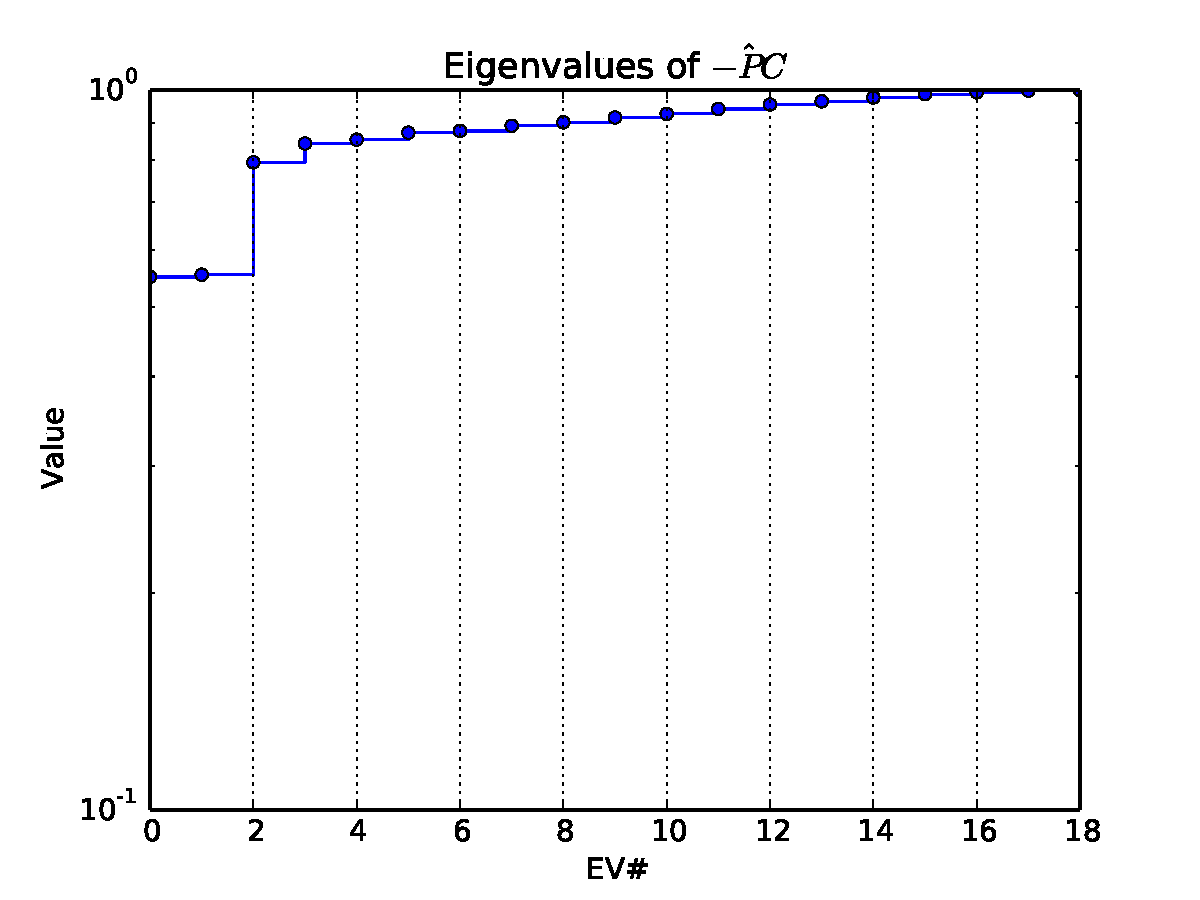
\includegraphics[width=.49\linewidth]{../EV[-C],problem=2,exact=0,N=32.pdf}
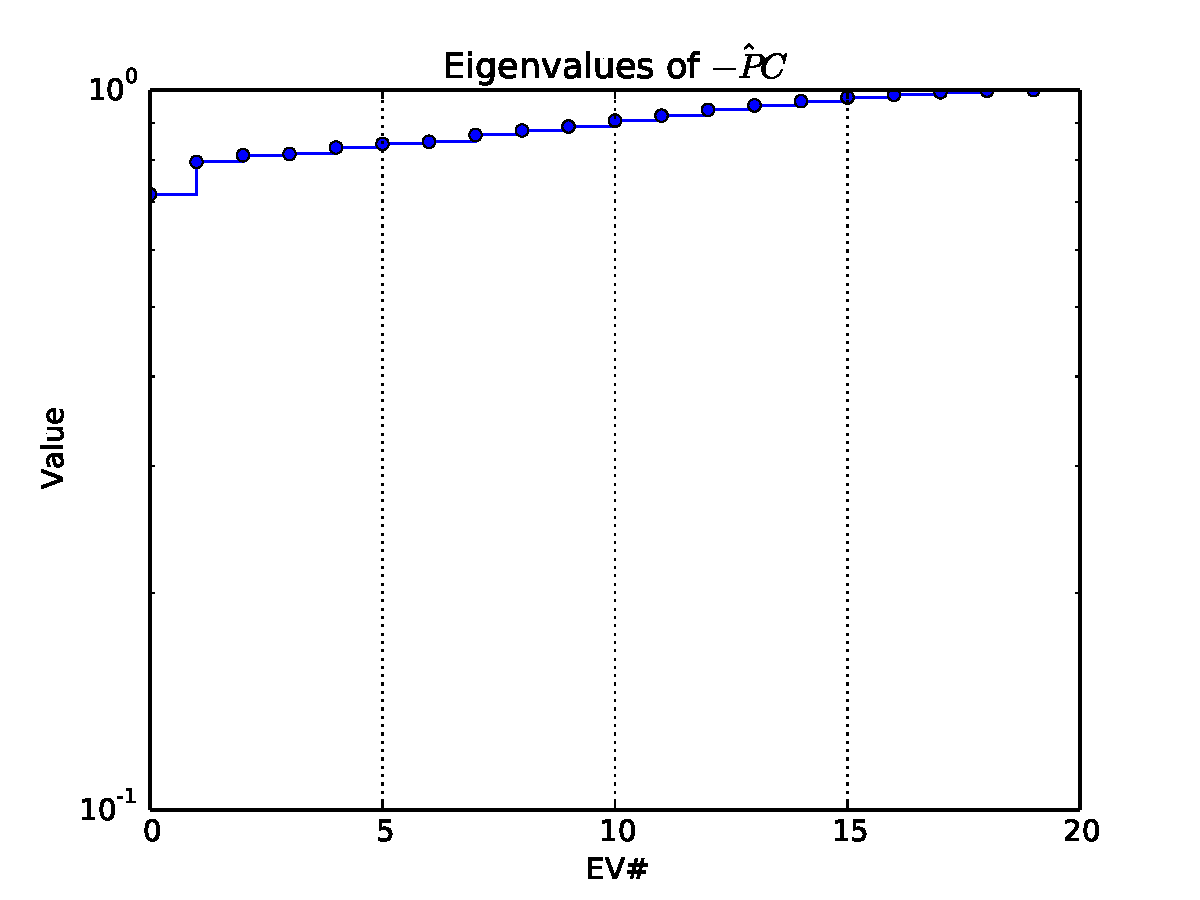
\includegraphics[width=.49\linewidth]{../EV[-C],problem=2,exact=0,N=64.pdf}
\caption{Eigenvalues of the preconditioned $-C$ block at $N=32$ (left) and $N=64$ (right).}
\label{evC}
\end{center}
\end{figure}


\begin{figure}
\begin{center}
\includegraphics[width=.49\linewidth]{../EV[-S_c],problem=2,exact=0,N=32.pdf}
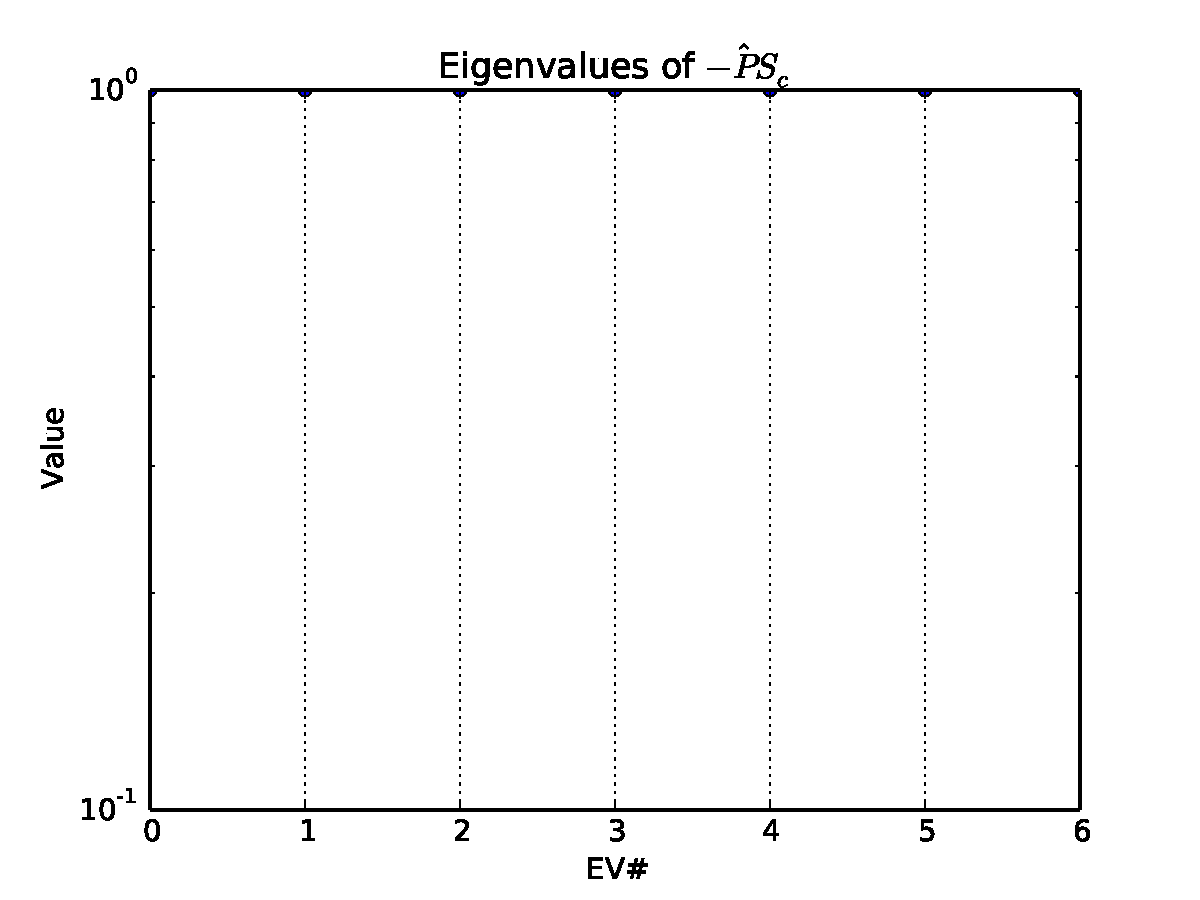
\includegraphics[width=.49\linewidth]{../EV[-S_c],problem=2,exact=0,N=64.pdf}
\caption{Eigenvalues of the preconditioned $-S_C$ block at $N=32$ (left) and $N=64$ (right).}
\label{evS}
\end{center}
\end{figure}

Figures \ref{evA}--\ref{evS} shows the preconditioned eigenvalues of the
preconditioned single blocks. Clearly, the eigenvalues here are nicely
bounded. We may here investigate how the number of ML sweeps affect the
eigenvalues.

This more or less concludes the discussion of the 2D spinal cord example. 

\FloatBarrier

\begin{figure}
\begin{center}
\includegraphics[page=36,width=\linewidth]{../../doc/presentation.pdf}
\caption{Contrast problem. There are differences in the parameters. Again $b=0$ everywhere (giving $\tau\rightarrow\infty$), and $\Delta t=10^{-3}$. Also, $p=0$ at the top, and $E$ is about $1/10$ of that shown here. These changes are arbitrary: I can create new figures with the same parameters if necessary.}
\label{contrast}
\end{center}
\end{figure}

The contrast example is shown in figure~\ref{contrast}. Figures~\ref{contrast-richardson} and~\ref{contrast-lgmres} show the convergence of Richardson and LGMRES on this example, and figures~\ref{contrast-evA}--\ref{contrast-evA} show the component eigenvalues.

Only the (Schur-based) fixed stress preconditioner is effective in this example. This is expected from earlier works: preconditioning based on the unmodified $C$ block does not work with high contrast. Furthermore, for the Fixed Stress method, the convergence is similar to the 2D spinal cord example for both Richardson and LGMRES.

The methods do NOT show any significant grid dependence. I did see grid dependence earlier, but that was probably (mostly) caused by the ILU preconditioner on the $C$/$S_C$ block.

\emph{JBH: Can we drop everything except fixed stress in the rest of the examples?}


\begin{figure}
\begin{center}
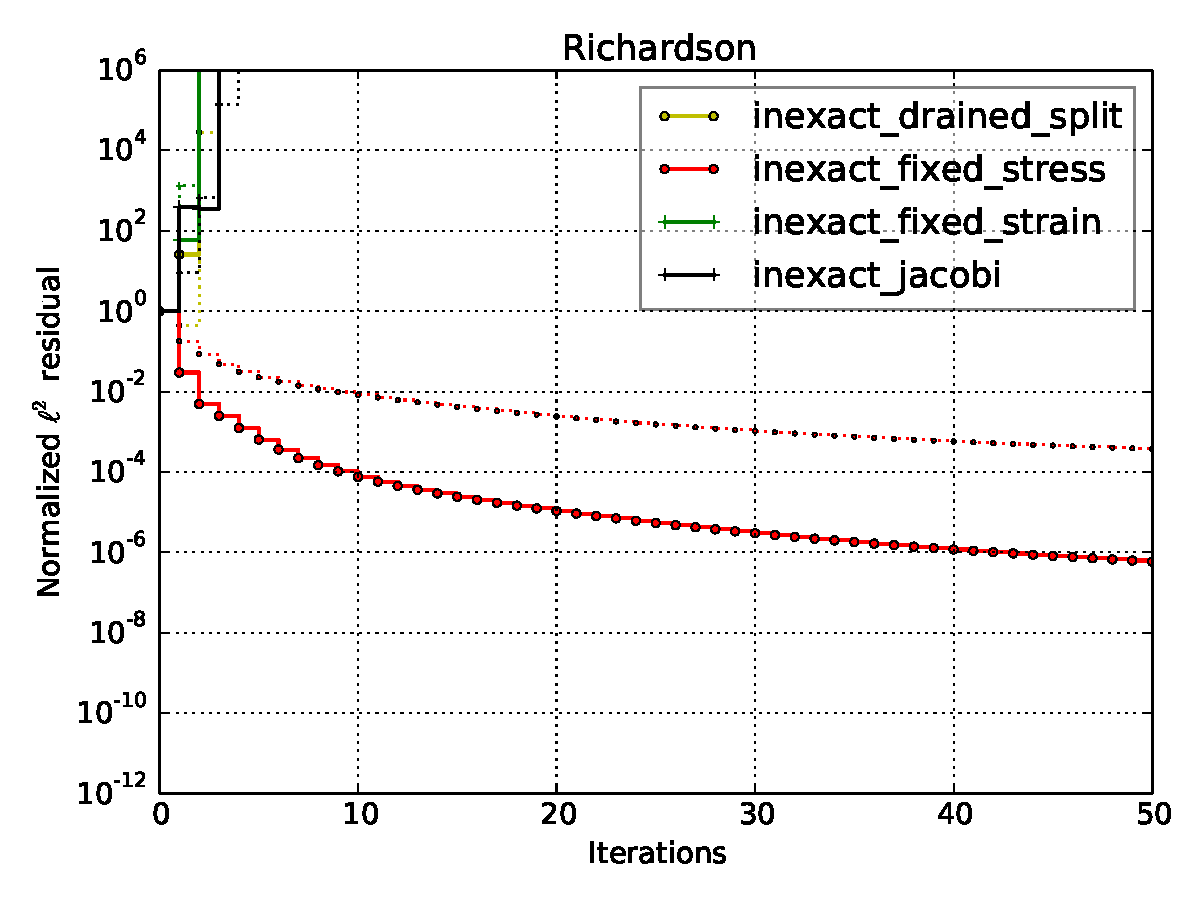
\includegraphics[width=0.49\linewidth]{../Richardson,problem=1,exact=0,N=40.pdf}
\includegraphics[width=0.49\linewidth]{../Richardson,problem=1,exact=0,N=160.pdf}
\caption{Contrast problem ($\delta=10^{-8}$), Richardson, $N=40$ (left) and $N=160$ (right).}
\label{contrast-richardson}
\end{center}
\end{figure}

\begin{figure}
\begin{center}
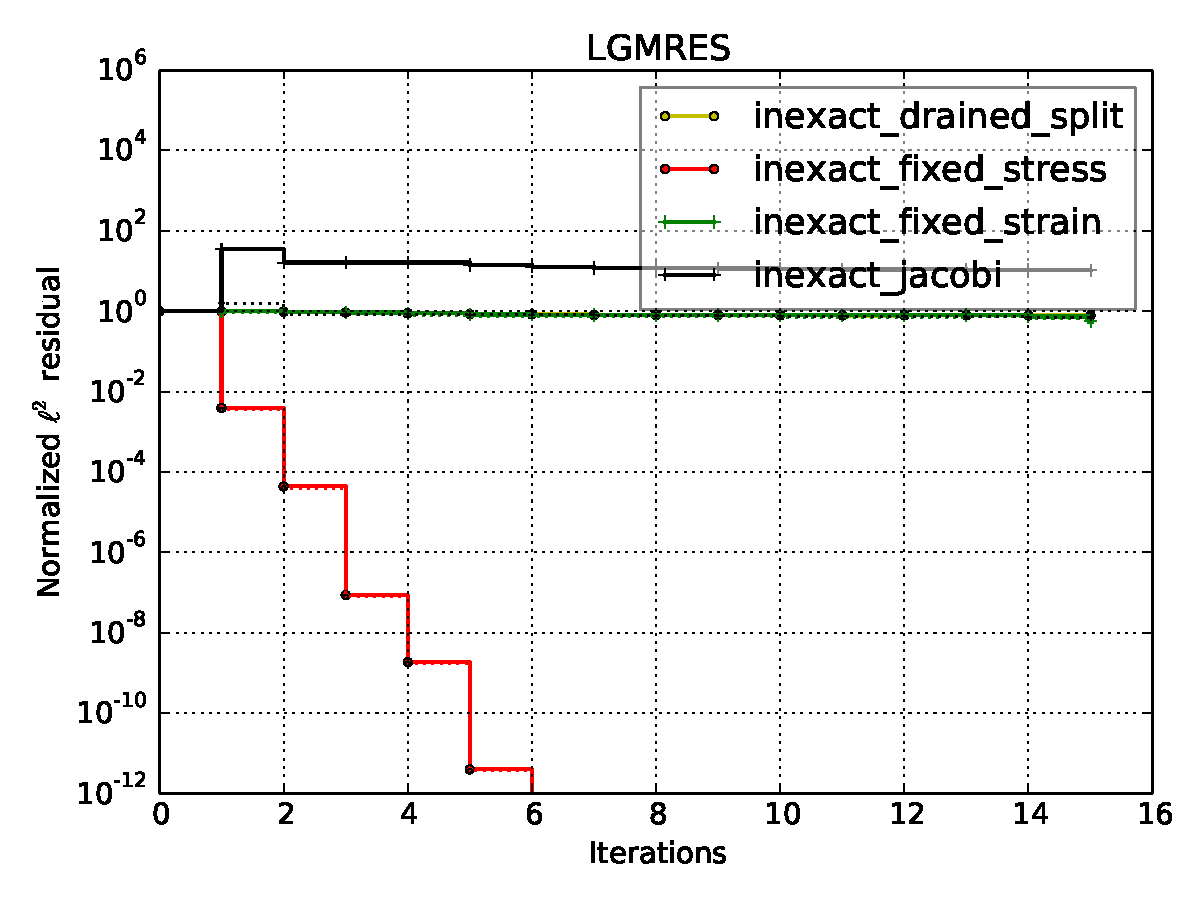
\includegraphics[width=0.49\linewidth]{../LGMRES,problem=1,exact=0,N=40,cycles=1.pdf}
\includegraphics[width=0.49\linewidth]{../LGMRES,problem=1,exact=0,N=160,cycles=1.pdf}
\caption{Contrast problem ($\delta=10^{-8}$), LGMRES, $N=40$ (left) and $N=160$ (right).}
\label{contrast-lgmres}
\end{center}
\end{figure}

\begin{figure}
\begin{center}
\includegraphics[width=0.49\linewidth]{../EV[A],problem=1,exact=0,N=40,cycles=2.pdf}
\includegraphics[width=0.49\linewidth]{../EV[A],problem=1,exact=0,N=160,cycles=2.pdf}
\caption{Contrast problem ($\delta=10^{-8}$). Eigenvalues, $N=40$ (left) and $N=160$ (right).}
\label{contrast-evA}
\end{center}
\end{figure}

\begin{figure}
\begin{center}
\includegraphics[width=0.49\linewidth]{../EV[-S_c],problem=1,exact=0,N=40,cycles=2.pdf}
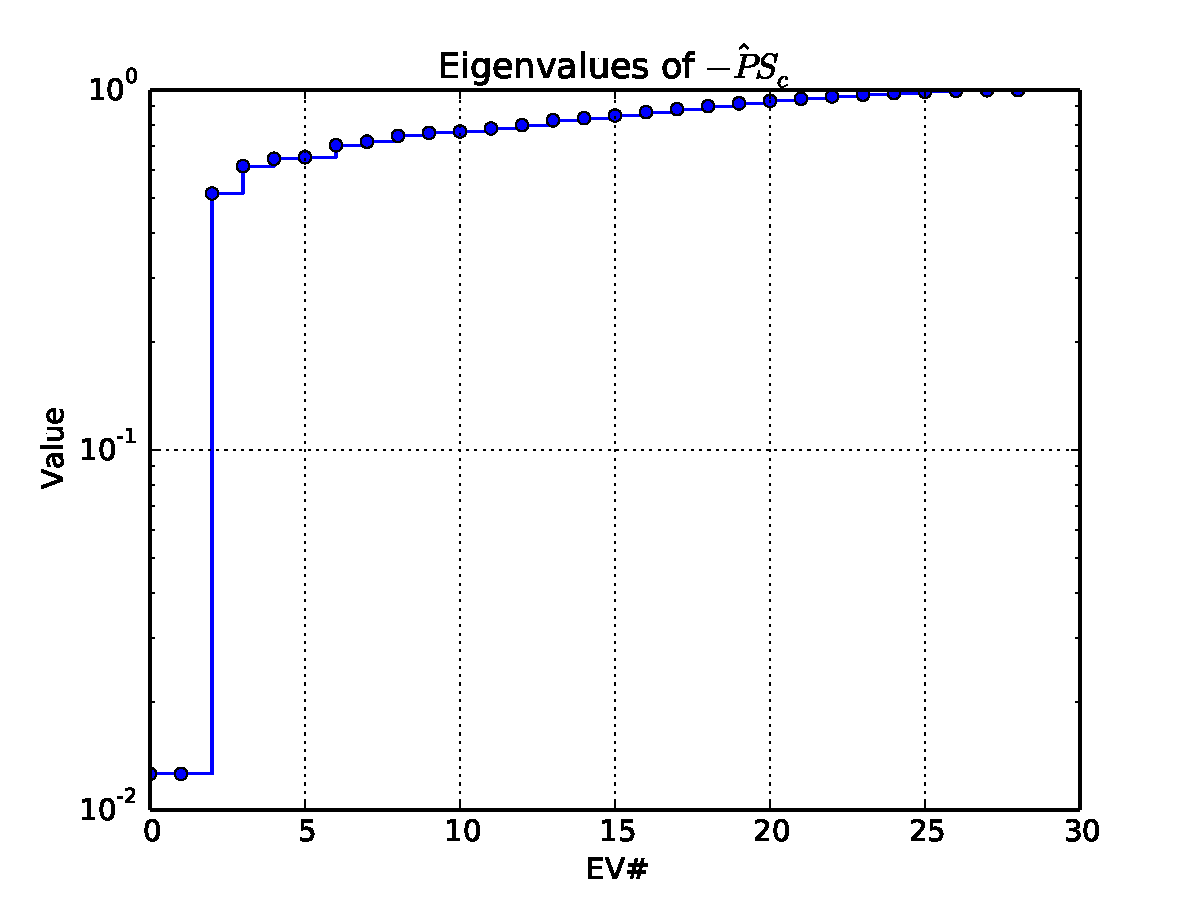
\includegraphics[width=0.49\linewidth]{../EV[-S_c],problem=1,exact=0,N=160,cycles=2.pdf}
\caption{Contrast problem ($\delta=10^{-8}$). Eigenvalues, $N=40$ (left) and $N=160$ (right).}
\end{center}
\label{contrast-evS}
\end{figure}

\FloatBarrier

When the contrast is increased to $10^{-12}$, something unexpected and bad happens with LGMRES: It fails to converge at high resolution, but the BiCGStab/Richardson methods don't! See figures~\ref{contrast12-richardson}--\ref{contrast12-lgmres}. My only guess is that this is some kind of numerical sensitivity in the LGMRES method. 

\emph{JBH: This is a nasty surprise. I don't know, maybe we should just forget about LGMRES and focus on BiCGStab after all. We can show decent and grid-independent results on BiCGStab, but we haven't got any ``killer'' examples.}

\begin{figure}
\begin{center}
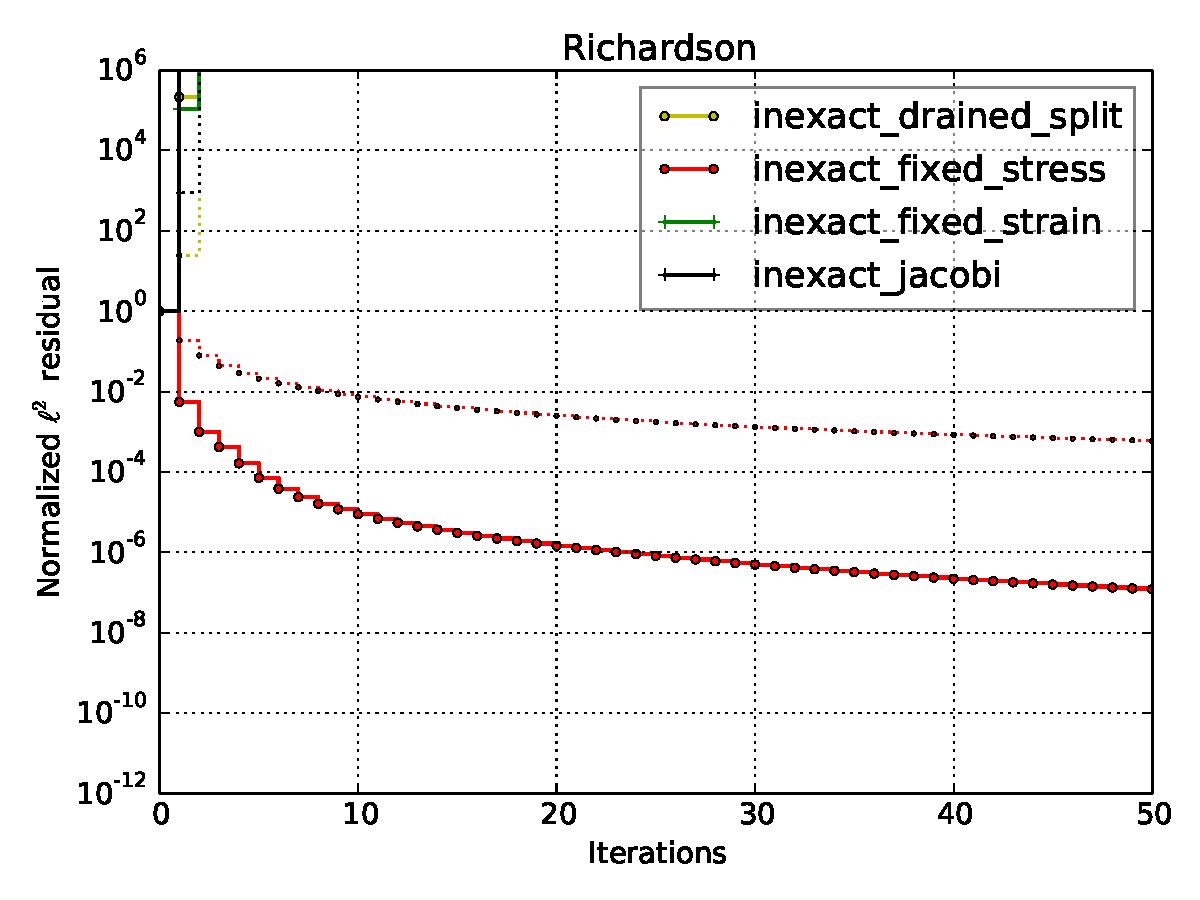
\includegraphics[width=0.49\linewidth]{../Richardson,problem=12,exact=0,N=40,cycles=2.pdf}
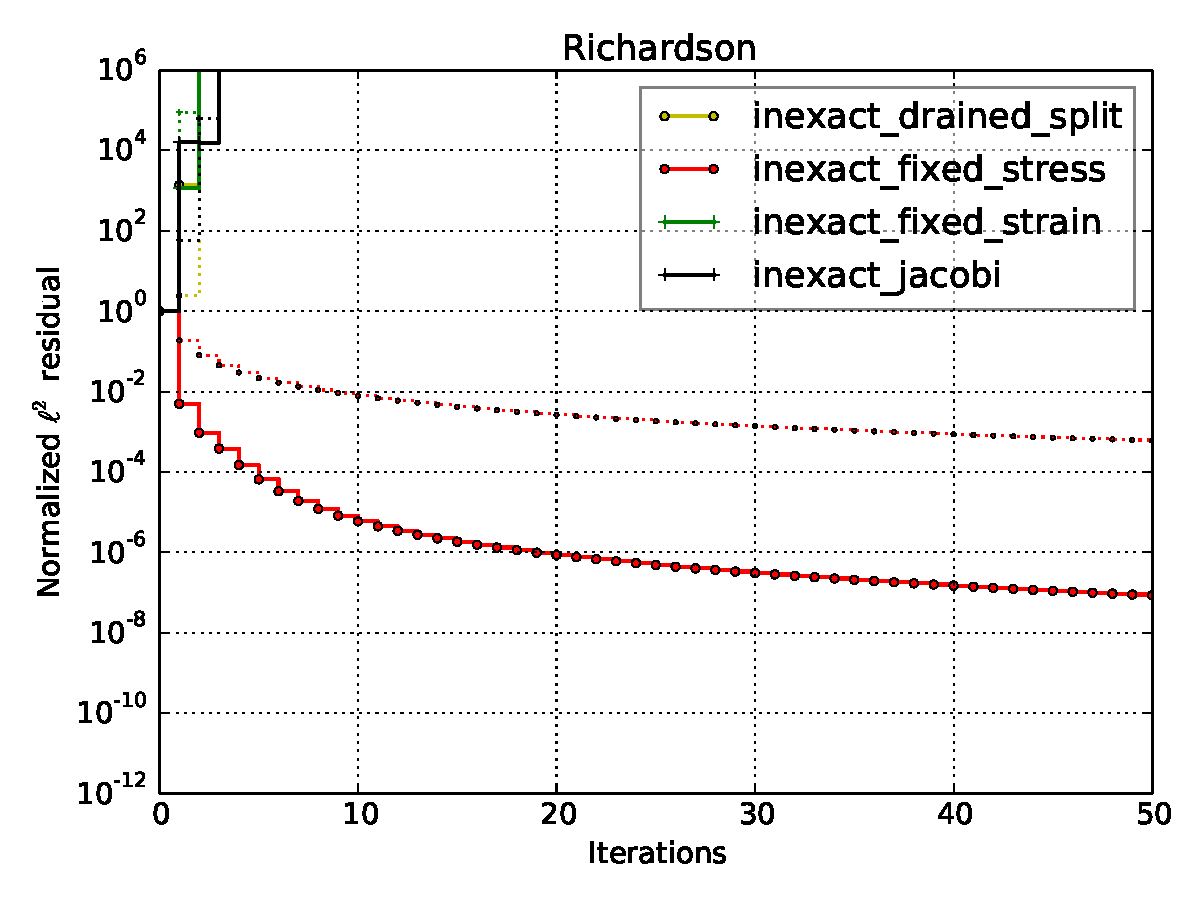
\includegraphics[width=0.49\linewidth]{../Richardson,problem=12,exact=0,N=640,cycles=2.pdf}
\caption{Contrast problem ($\delta=10^{-12}$), Richardson, $N=40$ (left) and $N=640$ (right). (NOTE: cycles=2)}
\label{contrast12-richardson}
\end{center}
\end{figure}

\begin{figure}
\begin{center}
\includegraphics[width=0.49\linewidth]{../BiCGStab,problem=12,exact=0,N=40,cycles=2.pdf}
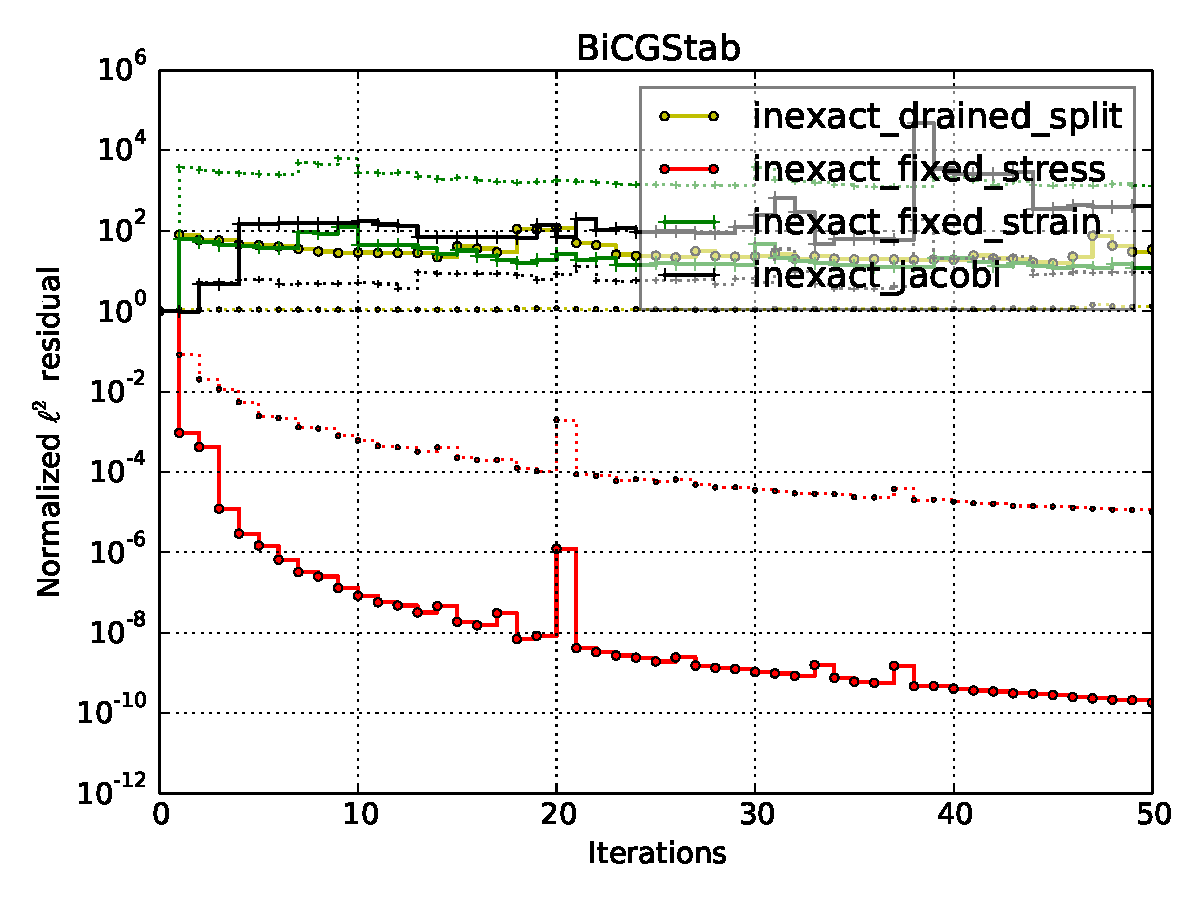
\includegraphics[width=0.49\linewidth]{../BiCGStab,problem=12,exact=0,N=640,cycles=2.pdf}
\caption{Contrast problem ($\delta=10^{-12}$), LGMRES, $N=40$ (left) and $N=640$ (right). (NOTE: cycles=2)}
\label{contrast12-bicgstab}
\end{center}
\end{figure}

\begin{figure}
\begin{center}
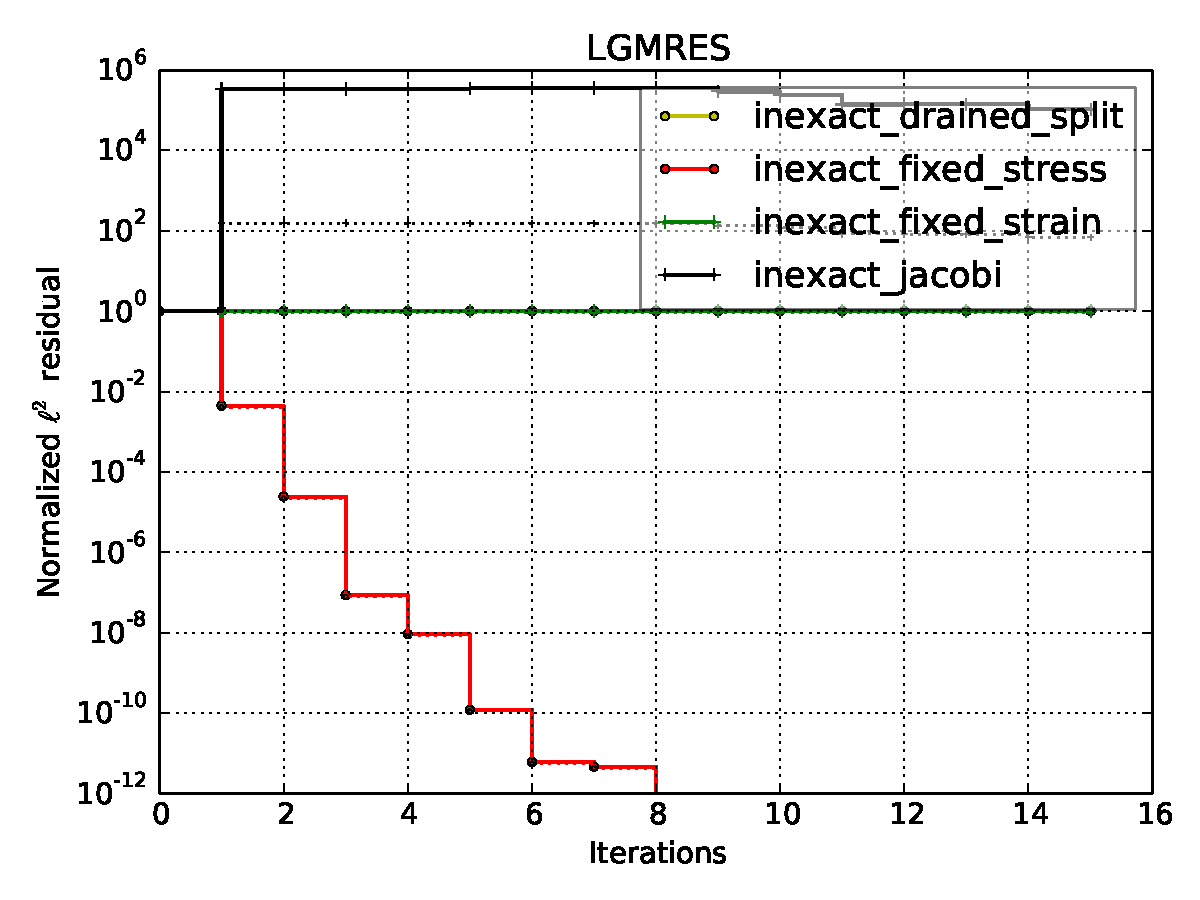
\includegraphics[width=0.49\linewidth]{../LGMRES,problem=12,exact=0,N=40,cycles=1.pdf}
\includegraphics[width=0.49\linewidth]{../LGMRES,problem=12,exact=0,N=640,cycles=1.pdf}
\caption{Contrast problem ($\delta=10^{-12}$), LGMRES, $N=40$ (left) and $N=640$ (right).}
\label{contrast12-lgmres}
\end{center}
\end{figure}

\begin{figure}
\begin{center}
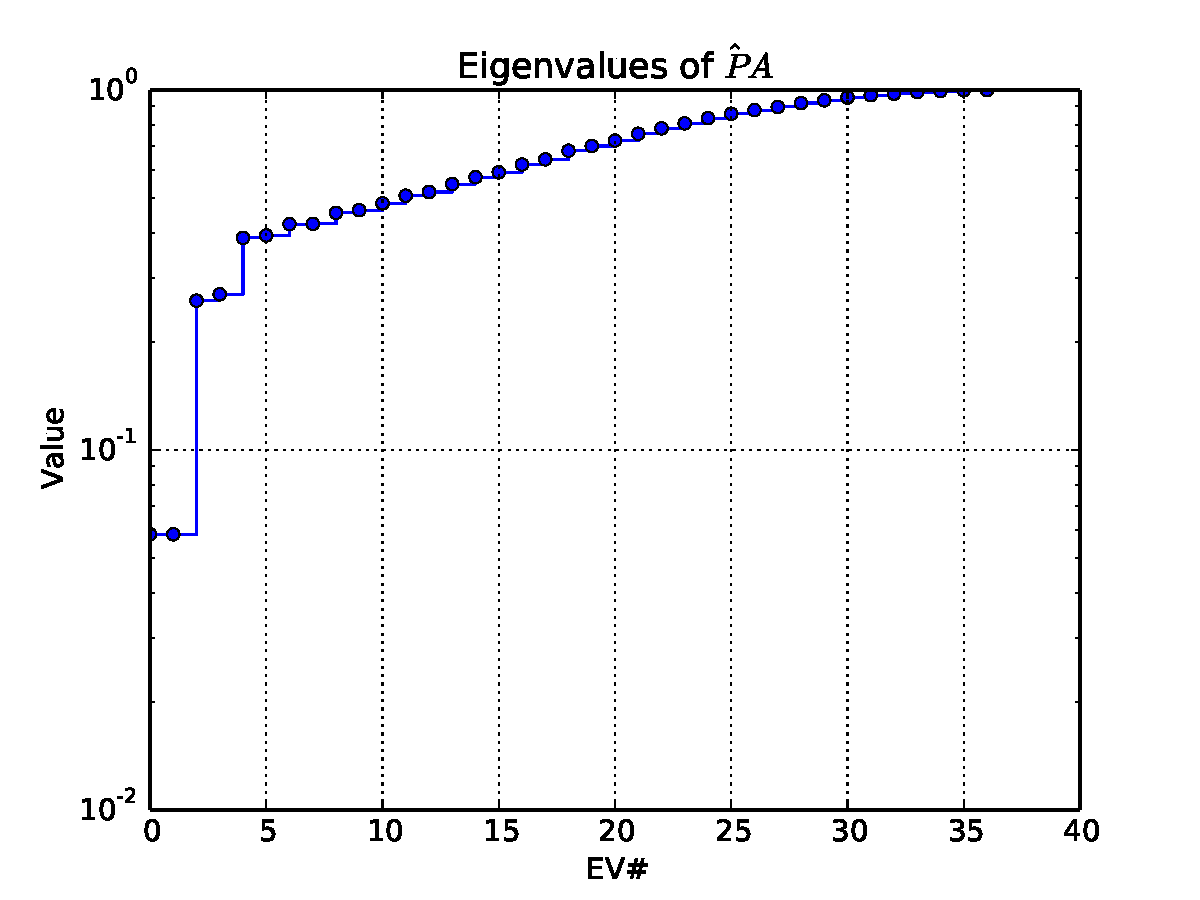
\includegraphics[width=0.49\linewidth]{../EV[A],problem=12,exact=0,N=40,cycles=2.pdf}
\includegraphics[width=0.49\linewidth]{../EV[A],problem=12,exact=0,N=640,cycles=2.pdf}
\caption{Contrast problem ($\delta=10^{-12}$). Eigenvalues, $N=40$ (left) and $N=640$ (right).}
\label{contrast12-evA}
\end{center}
\end{figure}

\begin{figure}
\begin{center}
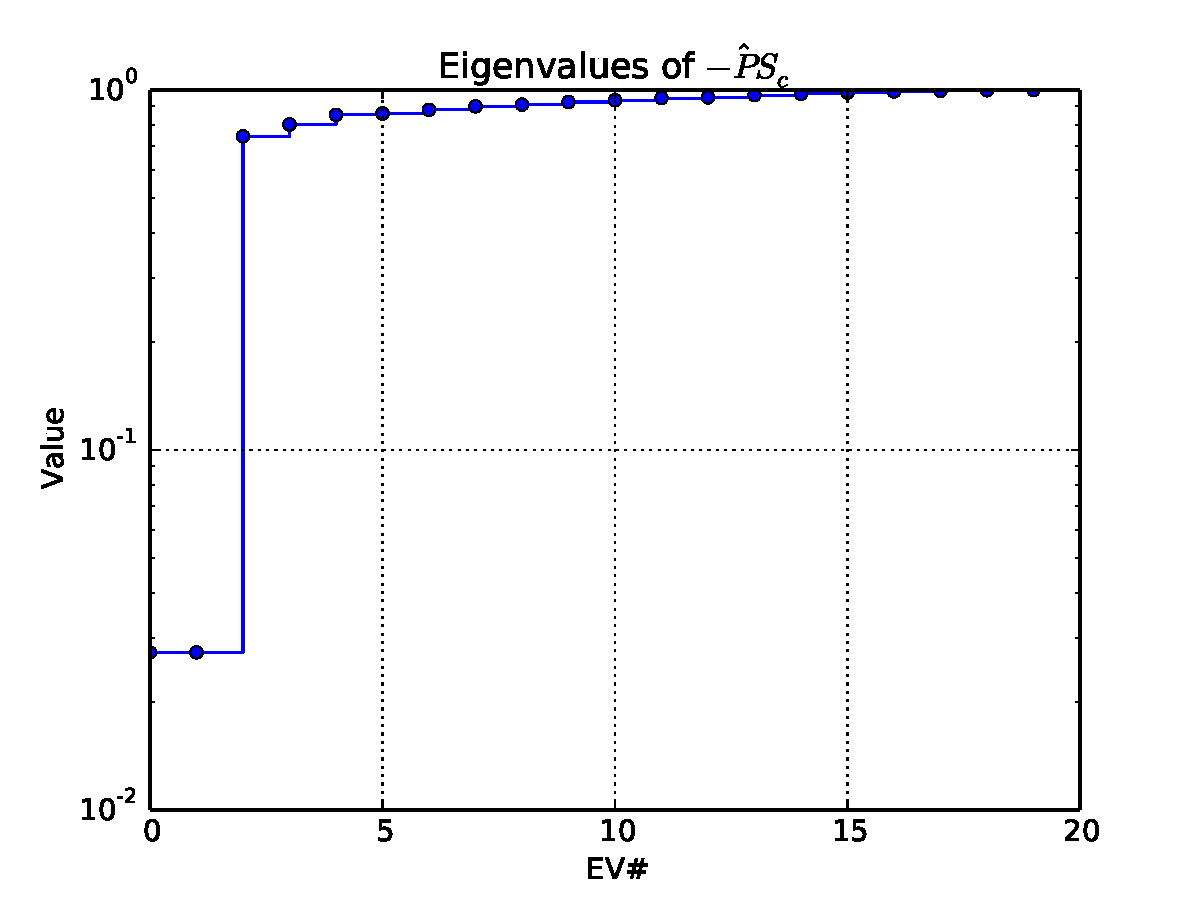
\includegraphics[width=0.49\linewidth]{../EV[-S_c],problem=12,exact=0,N=40,cycles=2.pdf}
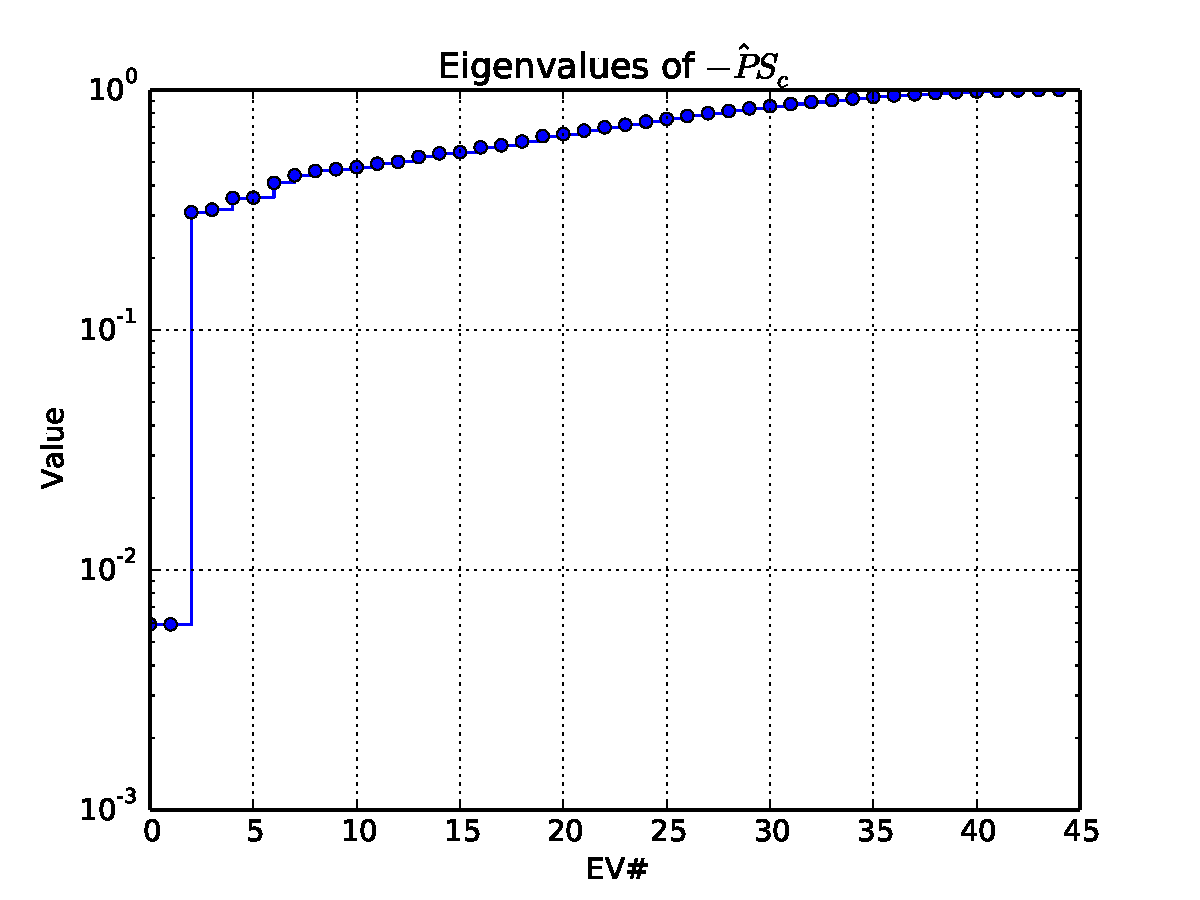
\includegraphics[width=0.49\linewidth]{../EV[-S_c],problem=12,exact=0,N=640,cycles=2.pdf}
\caption{Contrast problem ($\delta=10^{-12}$). Eigenvalues, $N=40$ (left) and $N=640$ (right).}
\end{center}
\label{contrast12-evS}
\end{figure}

\FloatBarrier

The end, for now. What follows is some new results with more iterations, in
order to have a more persuasive case for the advantage of the Krylov methods.

\begin{figure}
\begin{center}
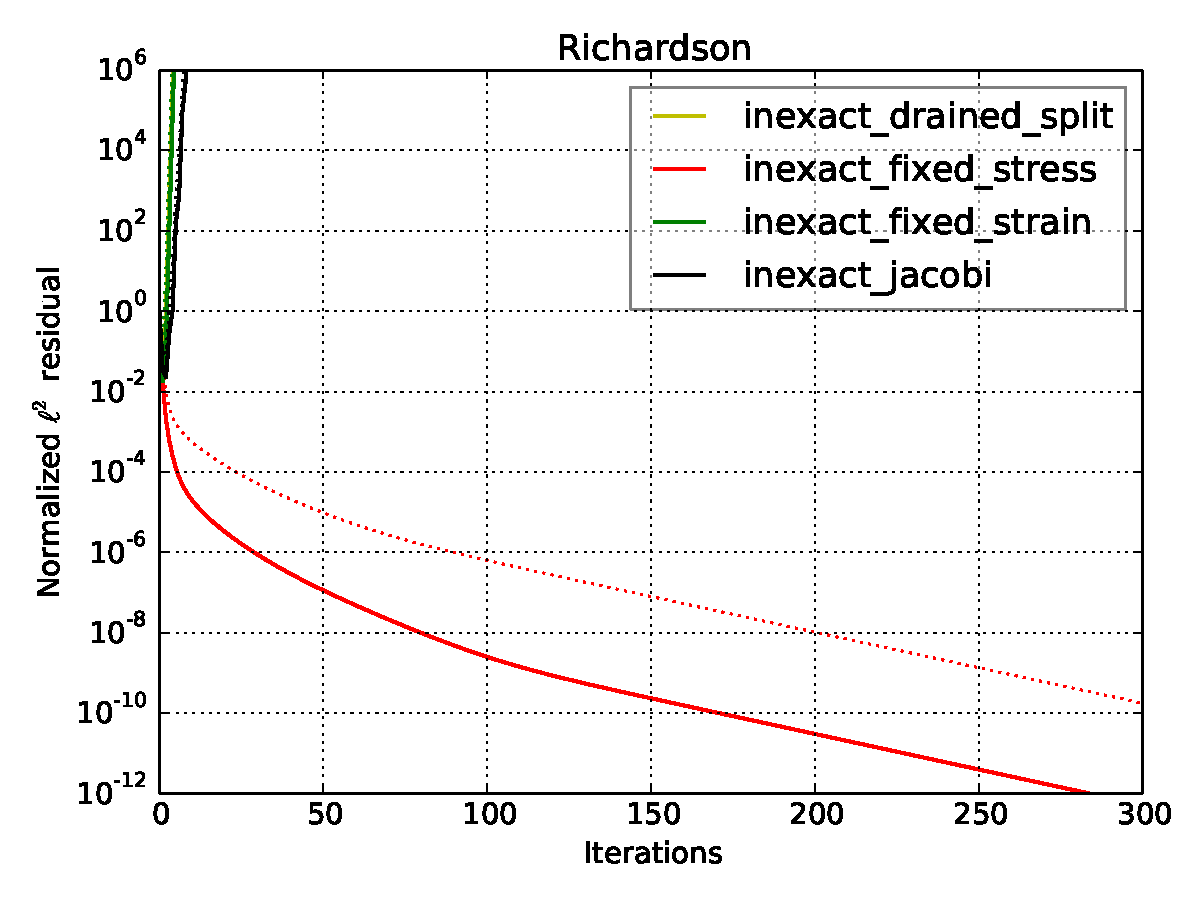
\includegraphics[width=0.32\linewidth]{../new-Richardson,problem=2,exact=0,N=64,cycles=1.pdf}
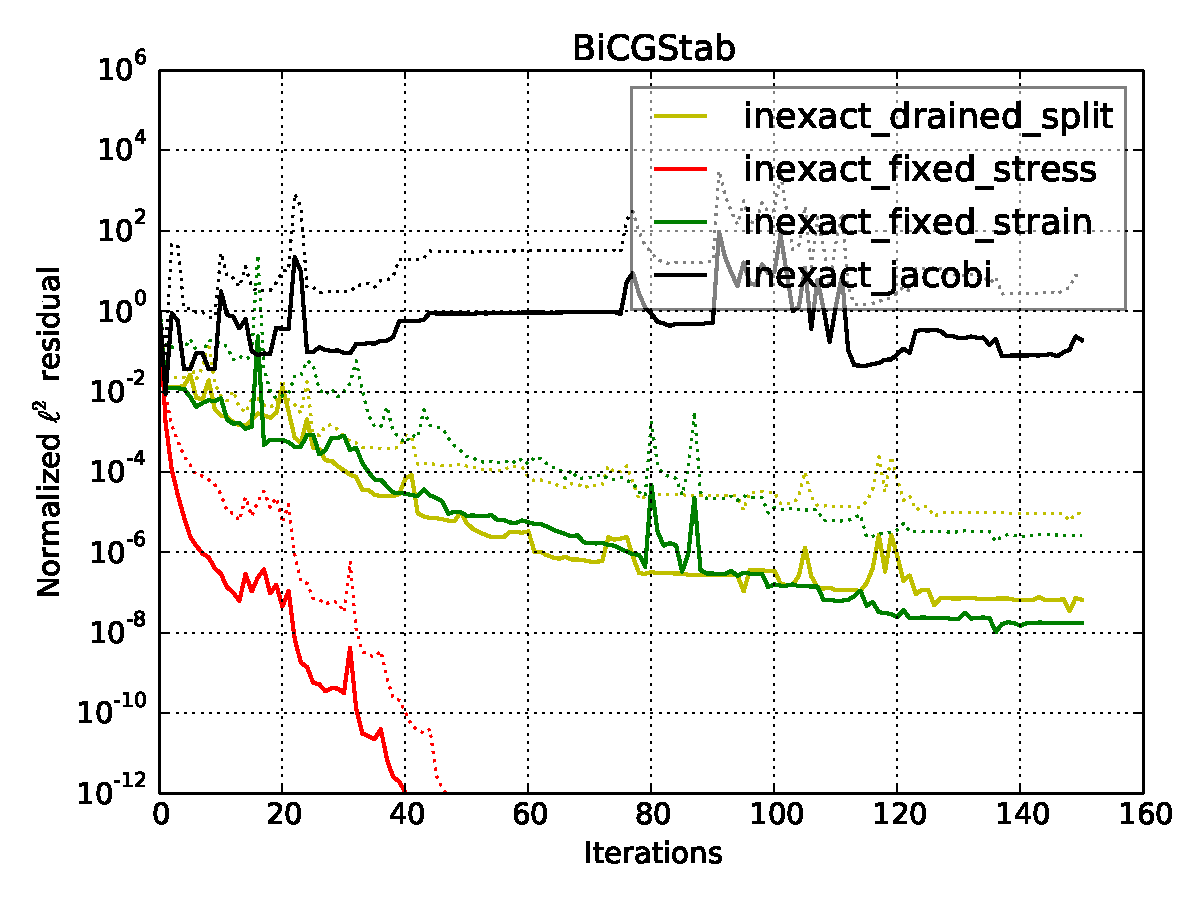
\includegraphics[width=0.32\linewidth]{../new-BiCGStab,problem=2,exact=0,N=64,cycles=1.pdf}
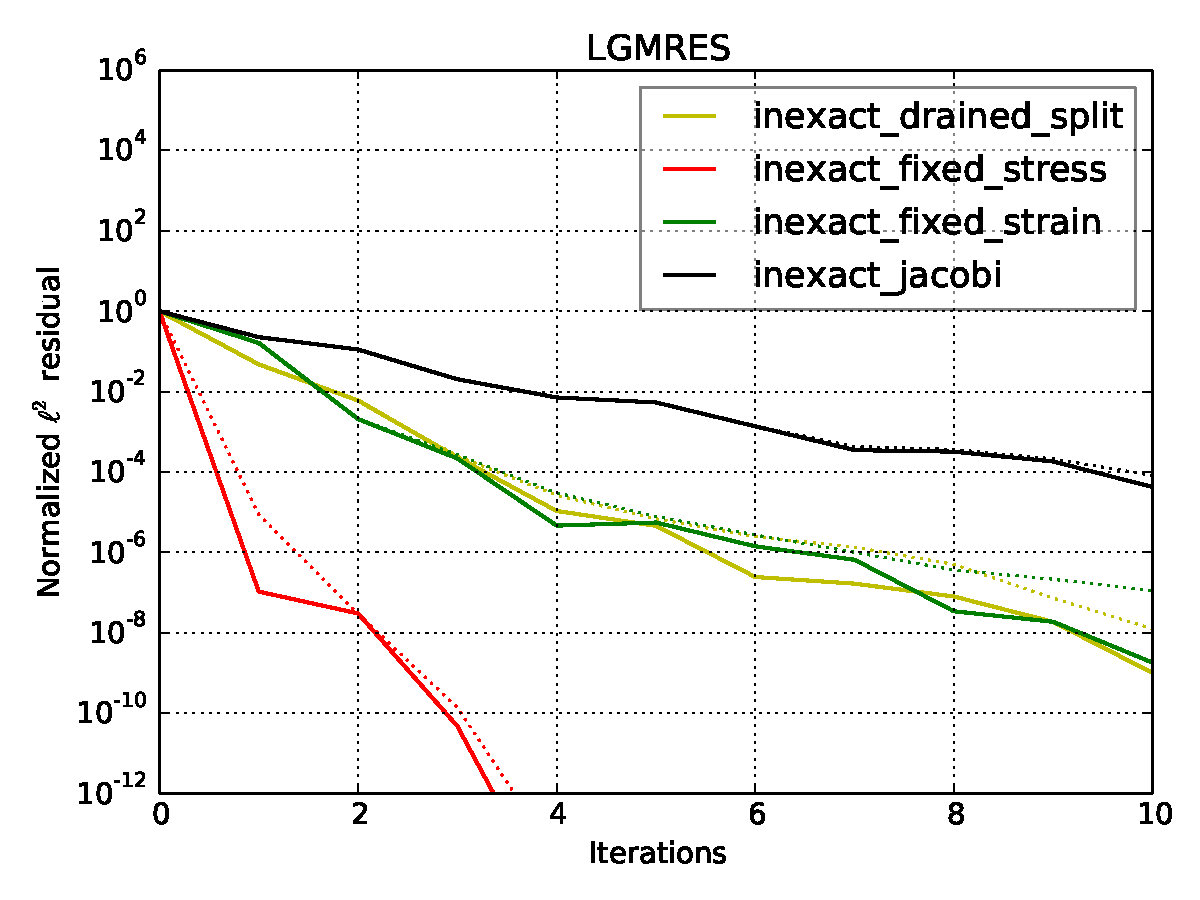
\includegraphics[width=0.32\linewidth]{../new-LGMRES,problem=2,exact=0,N=64,cycles=1.pdf}
\caption{Richardson, BiCGStab and LGMRES on the 2D spinal cord problem. The number of iterations is chosen to equalize the computing-time on the $x$ axis.} 
\label{new-2dsc-inexact}
\end{center}
\end{figure}


\begin{figure}
\begin{center}
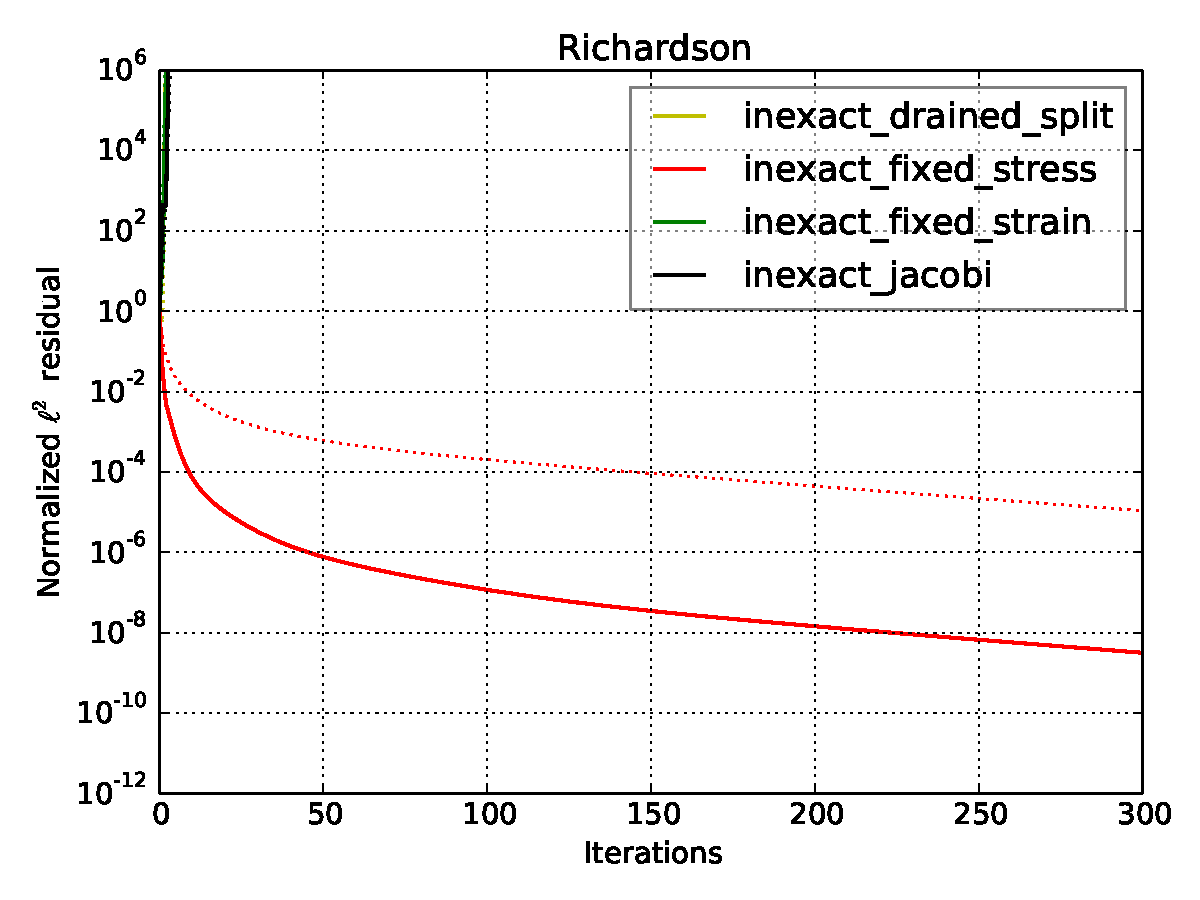
\includegraphics[width=0.49\linewidth]{../new-Richardson,problem=1,exact=0,N=40,cycles=1.pdf}
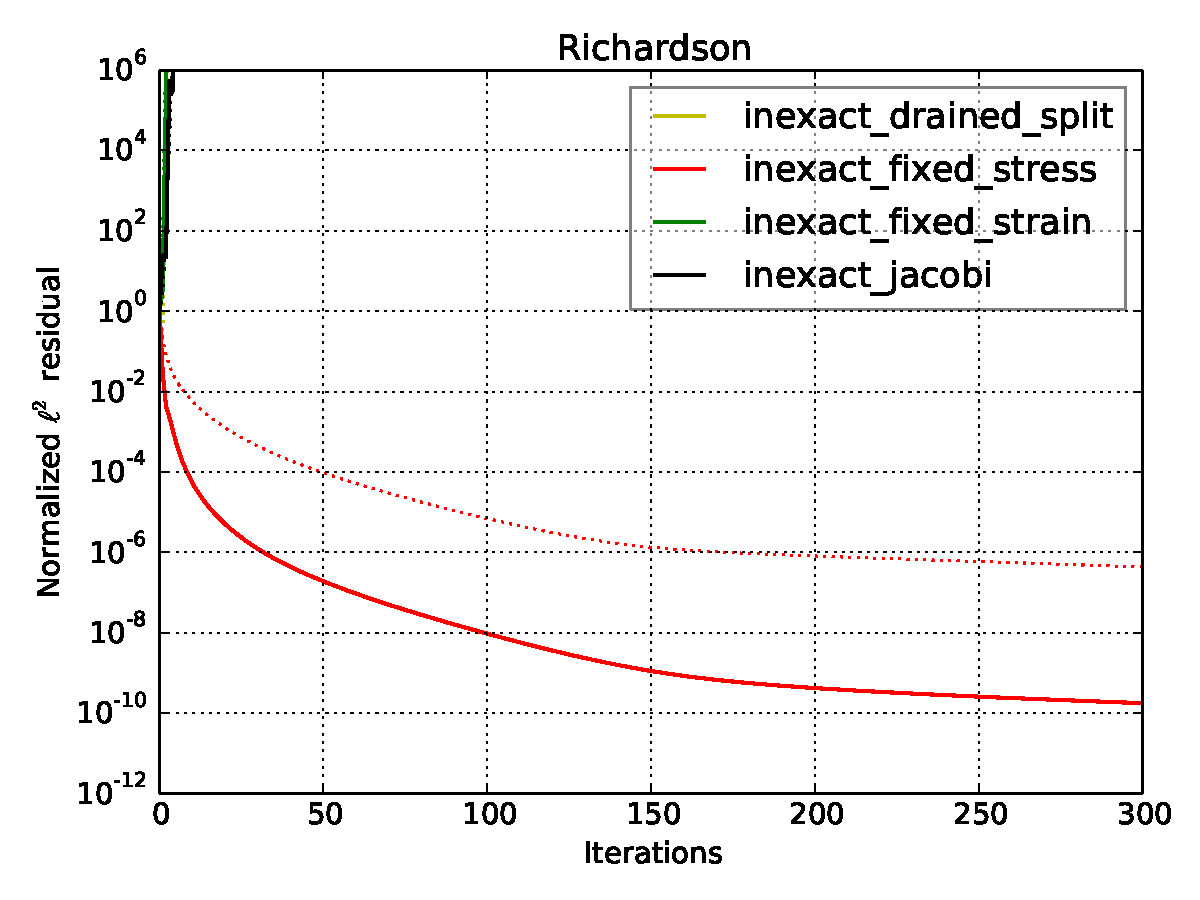
\includegraphics[width=0.49\linewidth]{../new-Richardson,problem=1,exact=0,N=160,cycles=1.pdf}
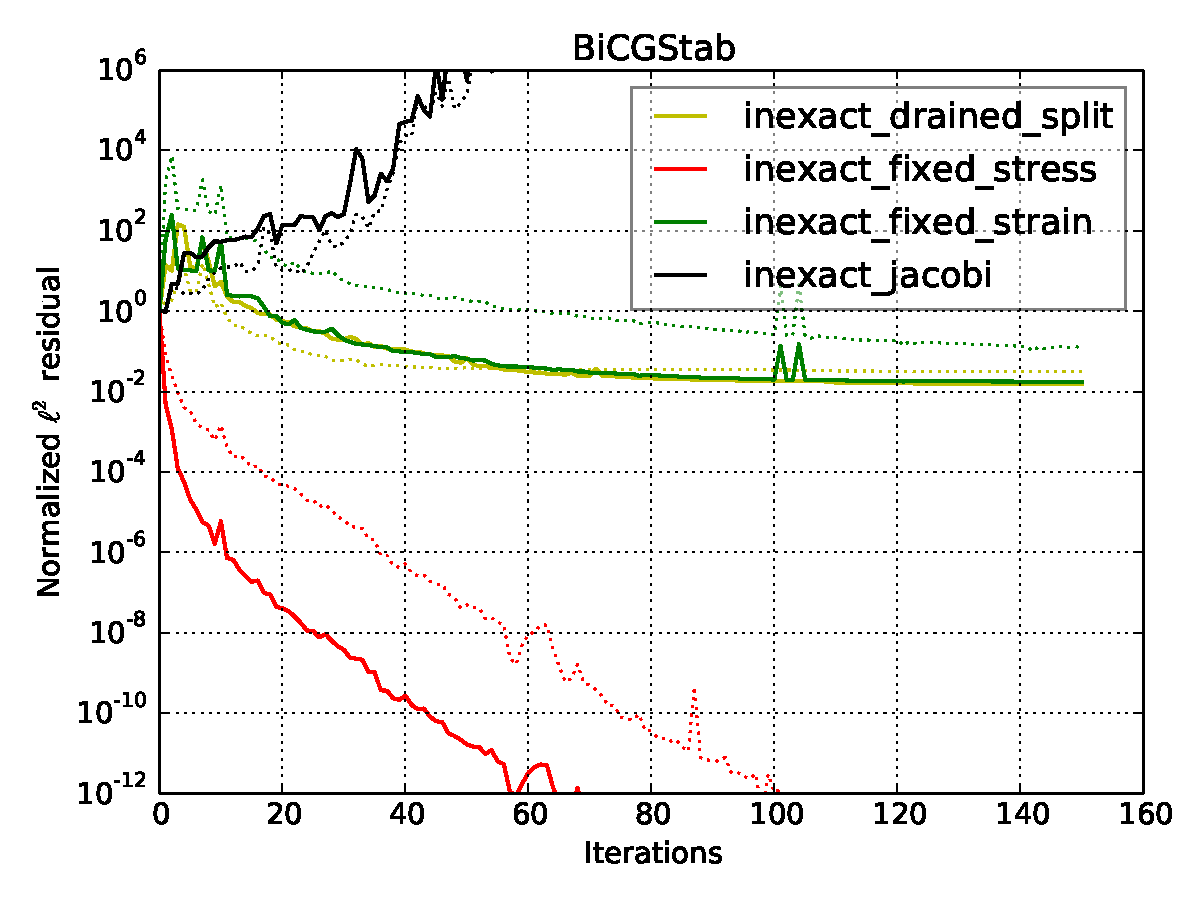
\includegraphics[width=0.49\linewidth]{../new-BiCGStab,problem=1,exact=0,N=40,cycles=1.pdf}
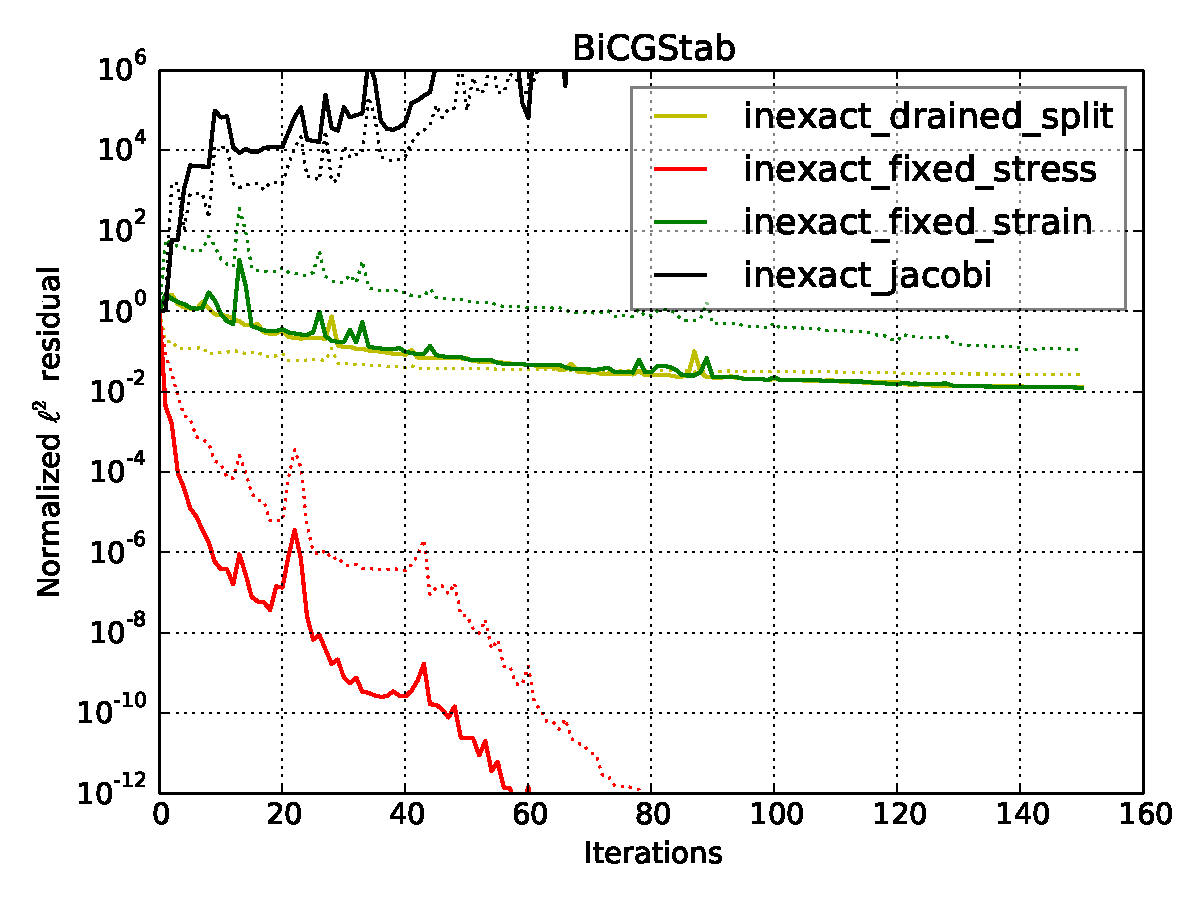
\includegraphics[width=0.49\linewidth]{../new-BiCGStab,problem=1,exact=0,N=160,cycles=1.pdf}
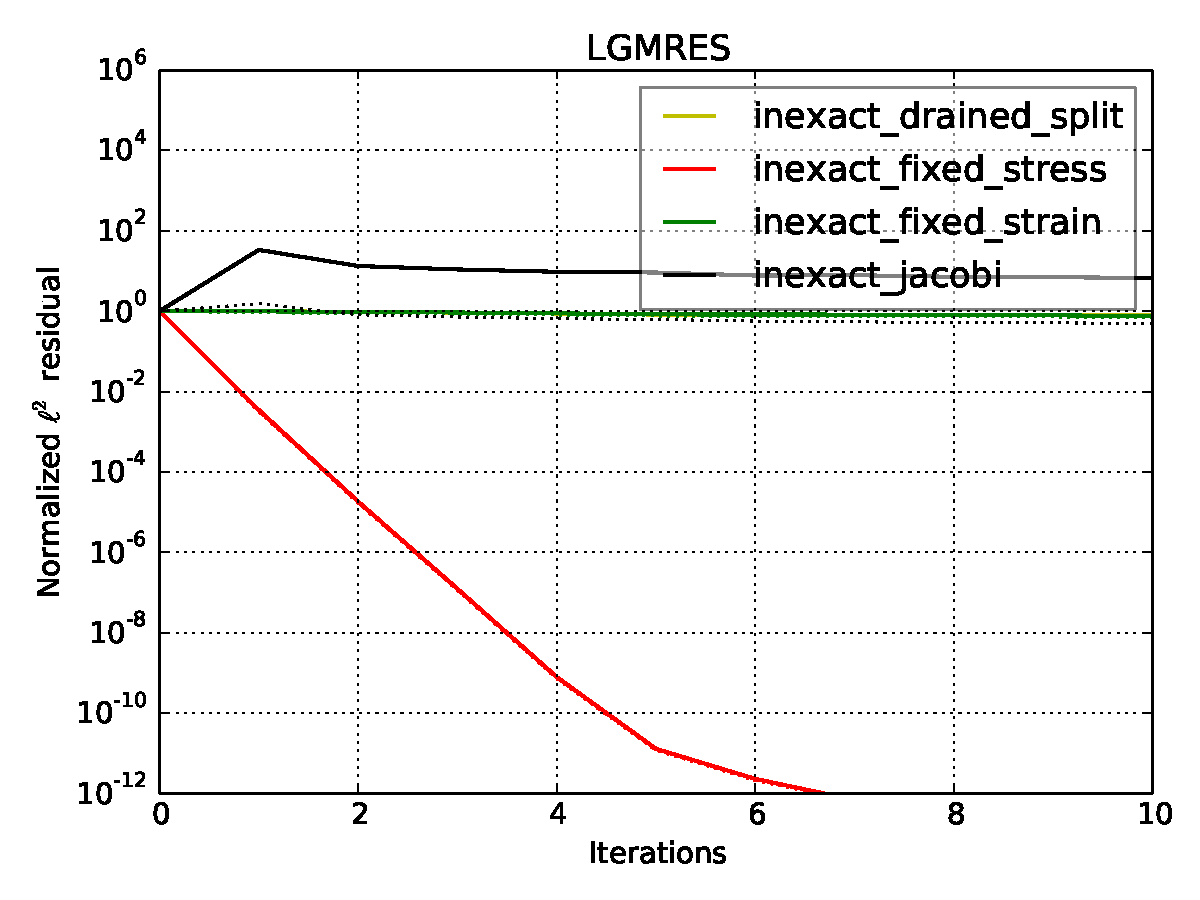
\includegraphics[width=0.49\linewidth]{../new-LGMRES,problem=1,exact=0,N=40,cycles=1.pdf}
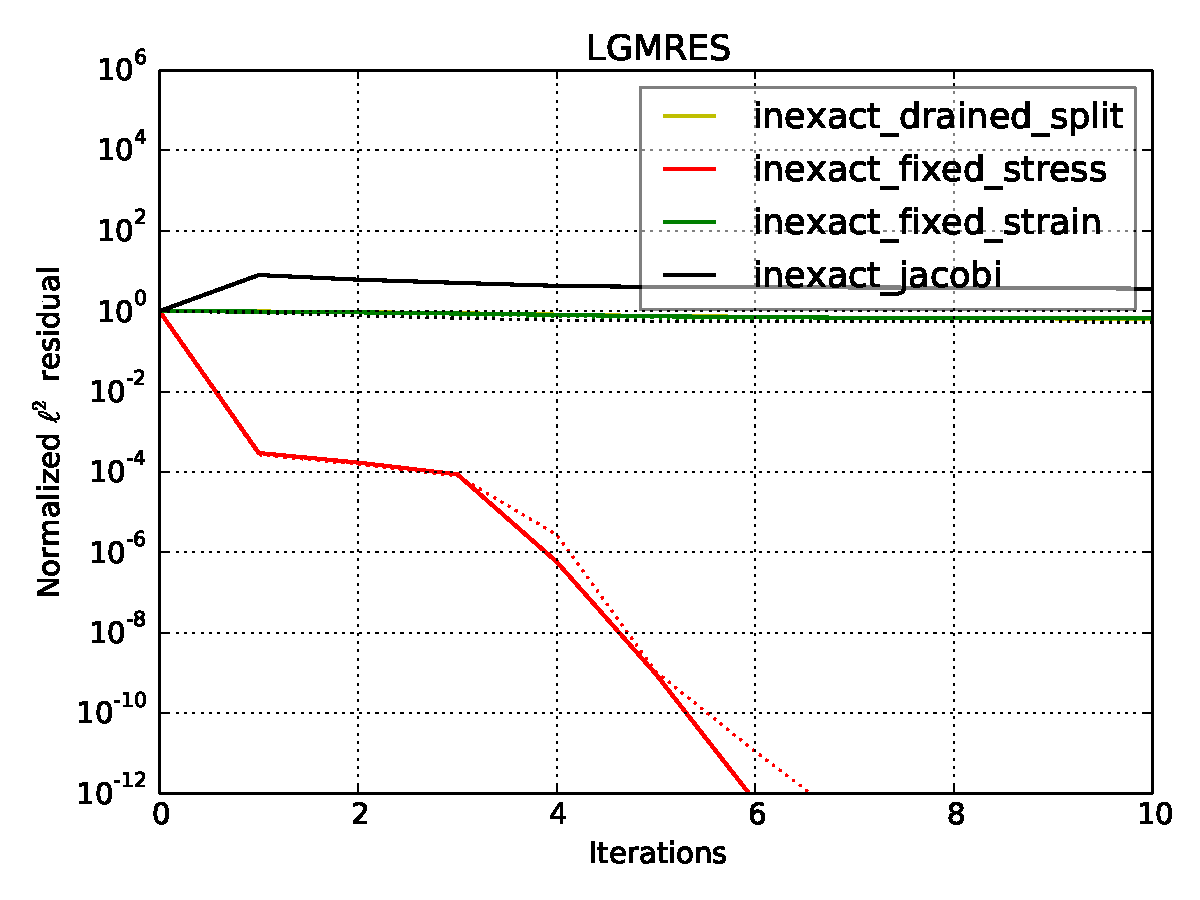
\includegraphics[width=0.49\linewidth]{../new-LGMRES,problem=1,exact=0,N=160,cycles=1.pdf}
\caption{Contrast problem ($\delta=10^{-8}$), LGMRES, $N=40$ (left) and $N=160$ (right).}
\label{contrast12-lgmres}
\end{center}
\end{figure}

\begin{figure}
\begin{center}
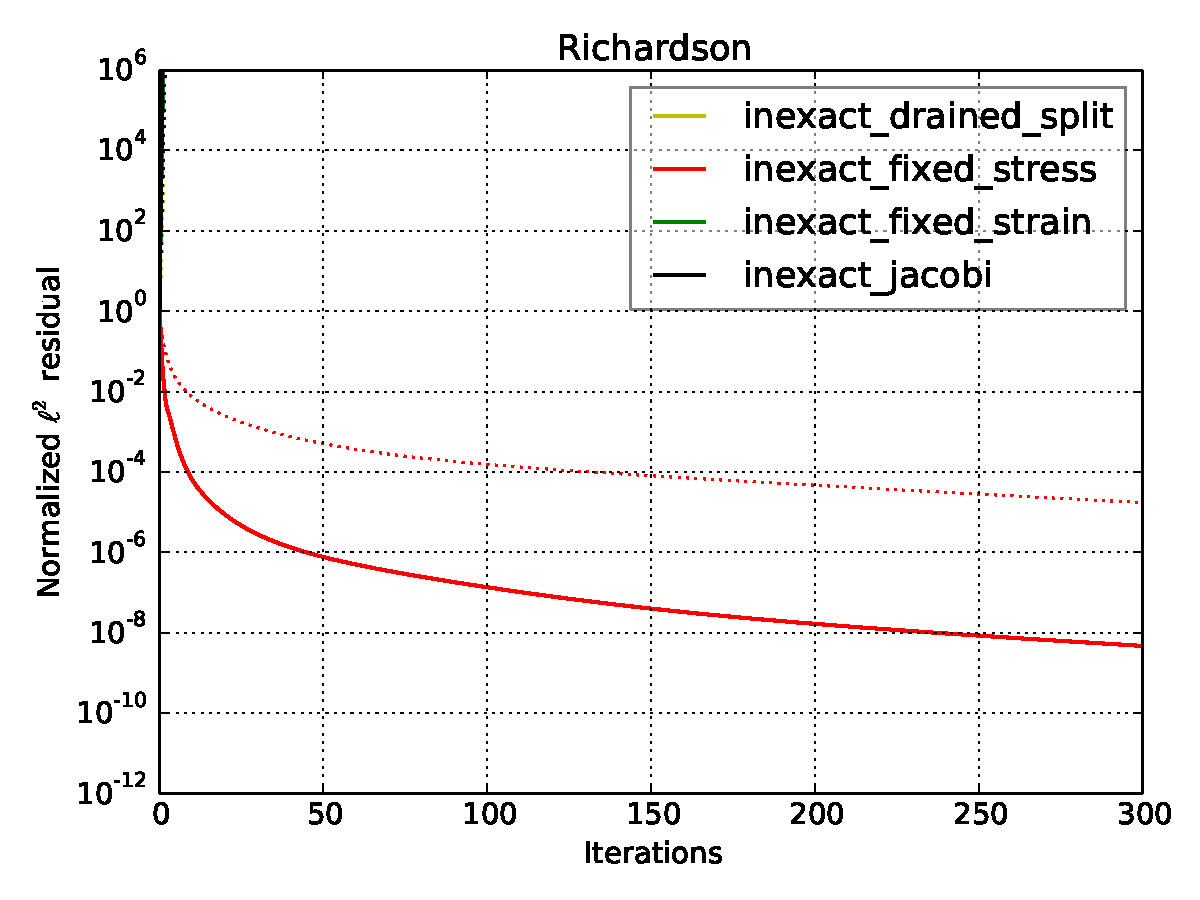
\includegraphics[width=0.49\linewidth]{../new-Richardson,problem=12,exact=0,N=40,cycles=1.pdf}
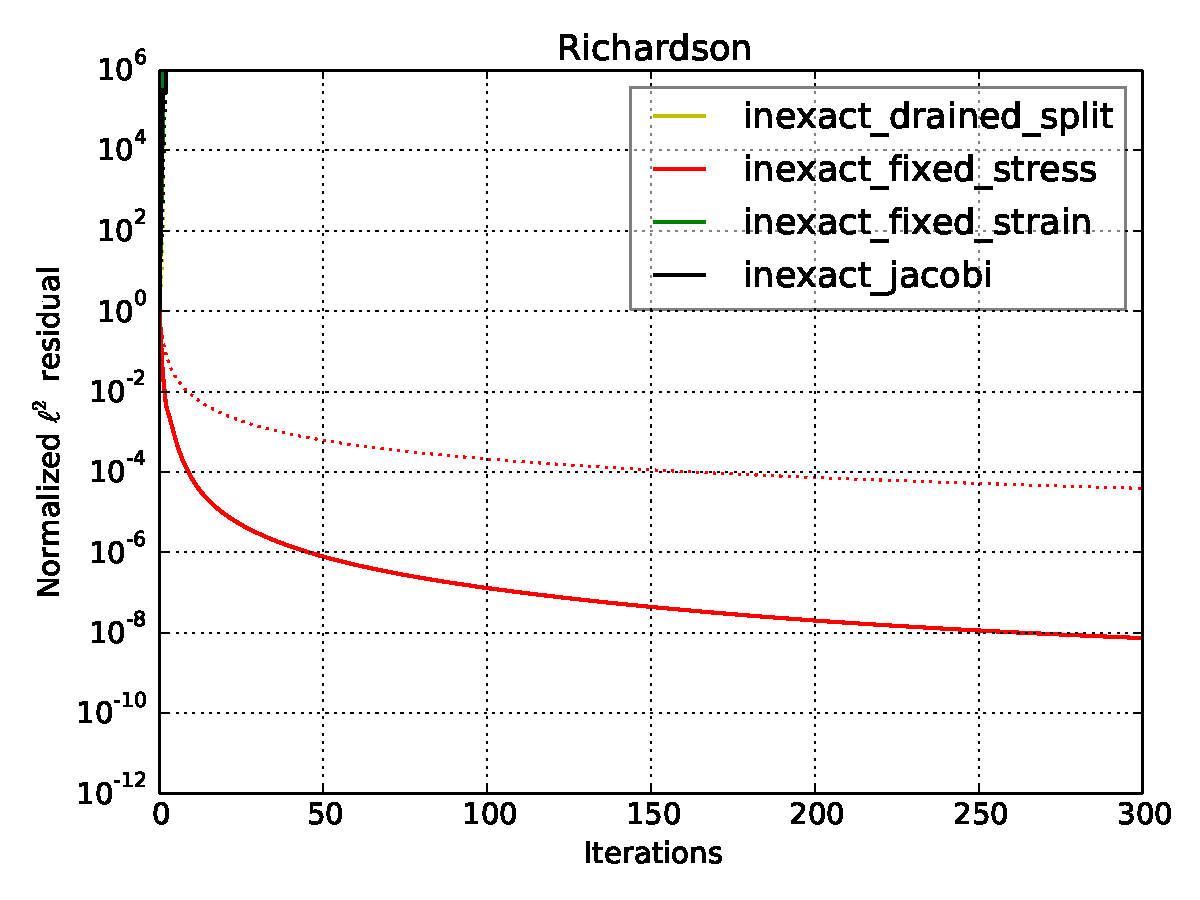
\includegraphics[width=0.49\linewidth]{../new-Richardson,problem=12,exact=0,N=160,cycles=1.pdf}
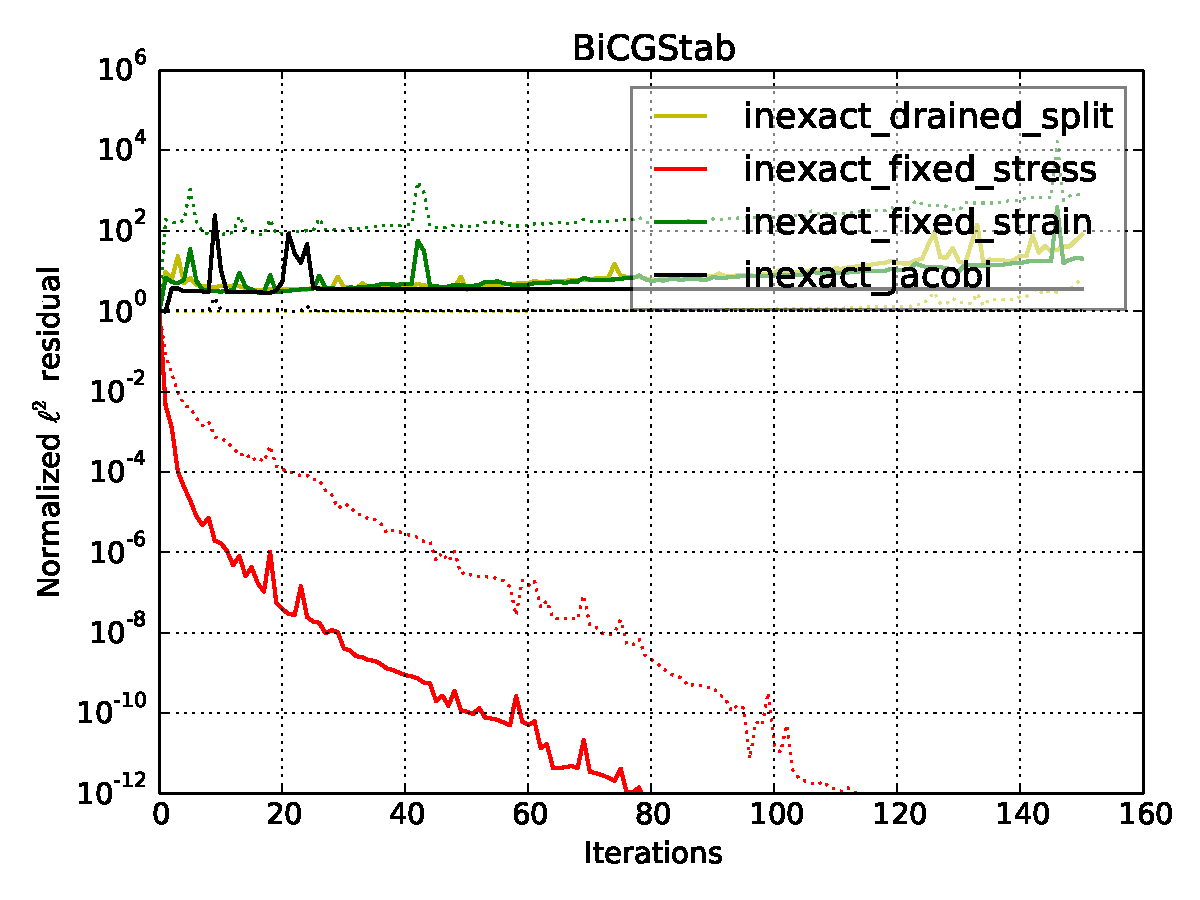
\includegraphics[width=0.49\linewidth]{../new-BiCGStab,problem=12,exact=0,N=40,cycles=1.pdf}
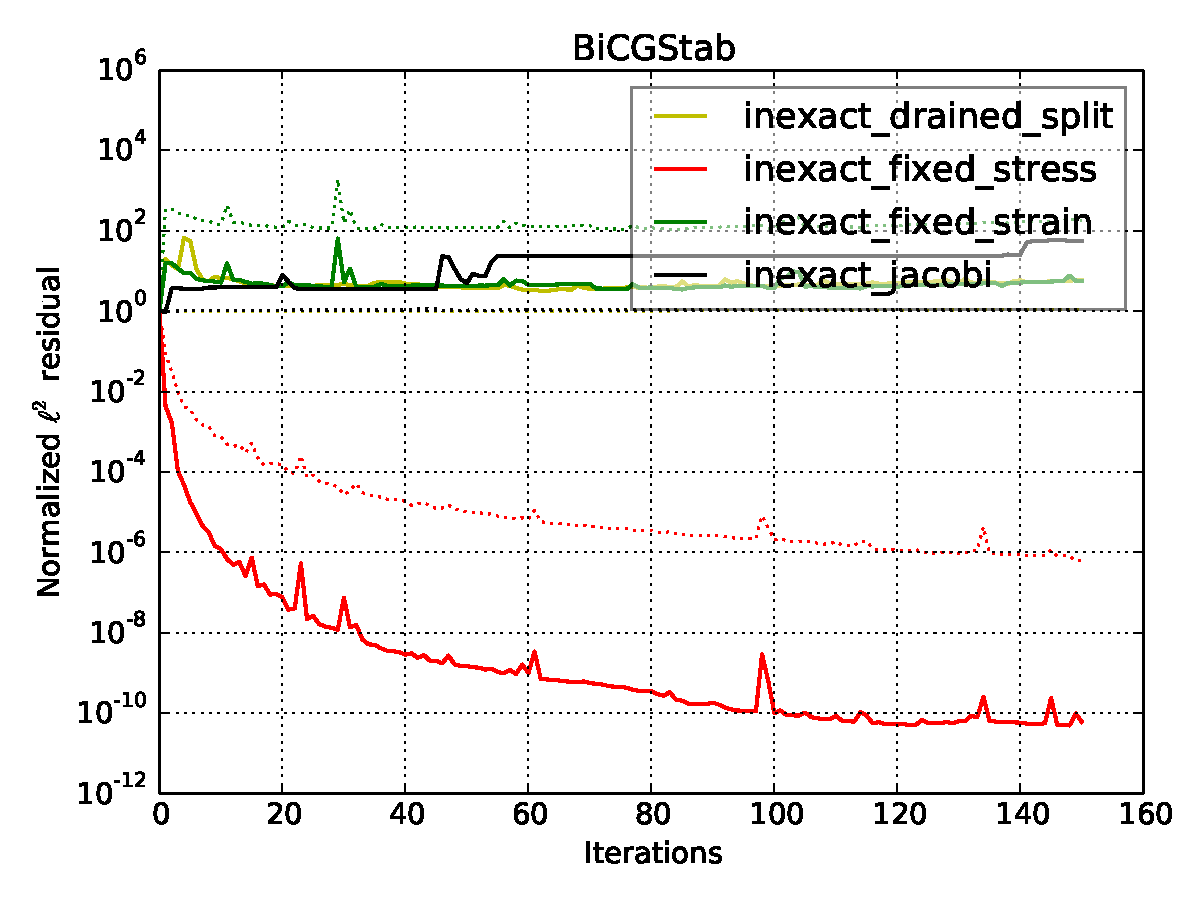
\includegraphics[width=0.49\linewidth]{../new-BiCGStab,problem=12,exact=0,N=160,cycles=1.pdf}
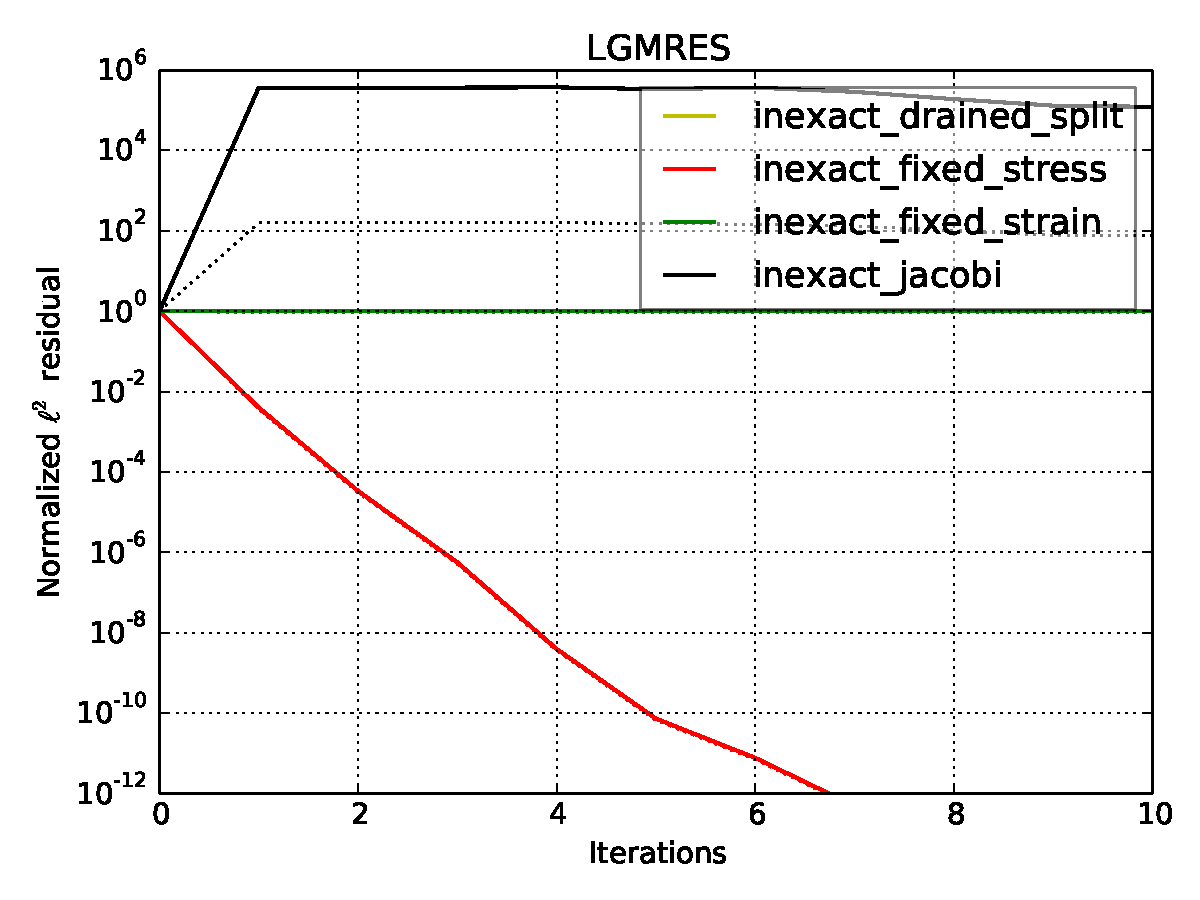
\includegraphics[width=0.49\linewidth]{../new-LGMRES,problem=12,exact=0,N=40,cycles=1.pdf}
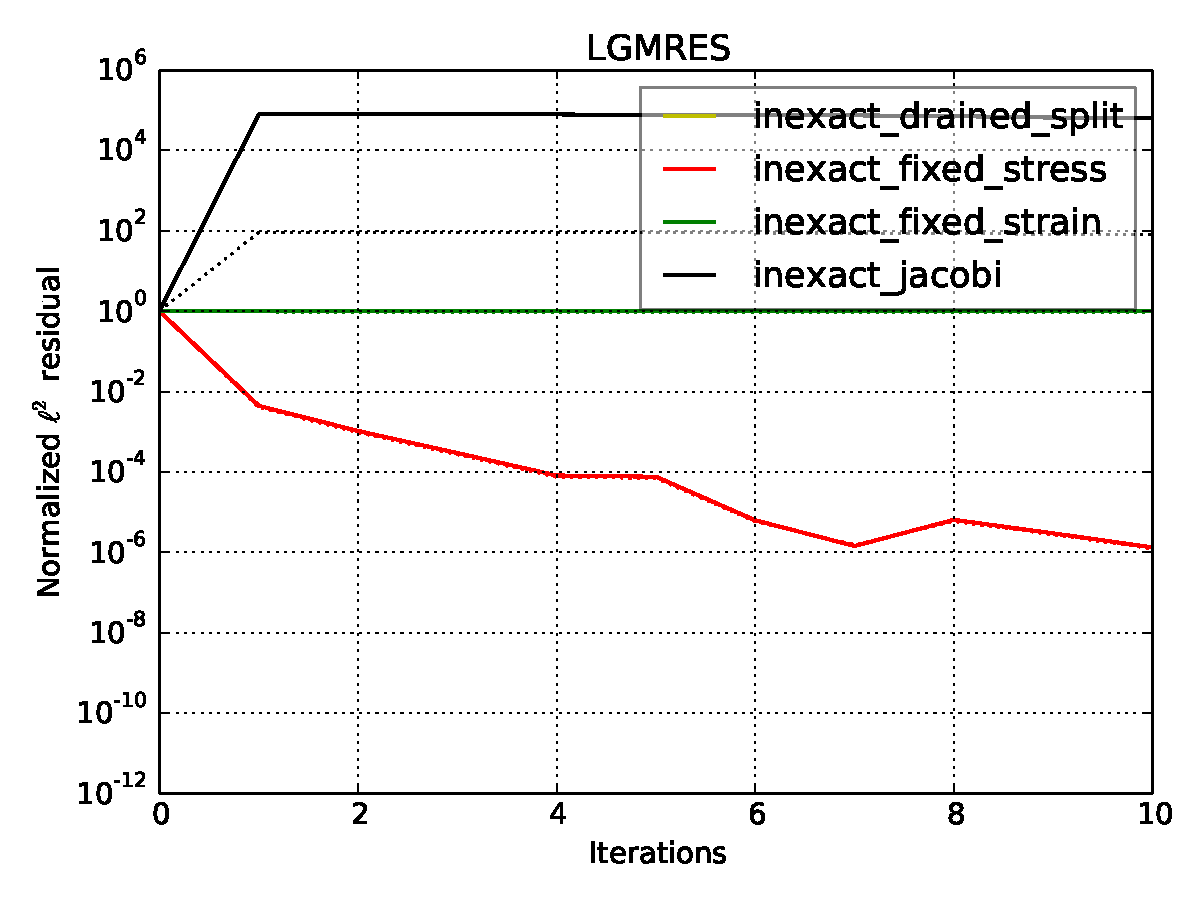
\includegraphics[width=0.49\linewidth]{../new-LGMRES,problem=12,exact=0,N=160,cycles=1.pdf}
\caption{Contrast problem ($\delta=10^{-12}$), LGMRES, $N=40$ (left) and $N=160$ (right).}
\label{contrast12-lgmres}
\end{center}
\end{figure}


\end{document}

